% TO-DO:
% * Actions = all possible transtions in RL
% * In RL, Q-learning is still unclear -- currently I'm using NN = transition F(x)
%   -- U(x) -> U(x') so it seems that generalization can occur in Q-space (?)
% * Structure of the turnstile is an important feature of the transition F(x)
% * Explain difference with AIXI
% * "inward" vs "outward"

\documentclass[orivec]{llncs}
\usepackage{graphicx}
\usepackage{amsmath}		% for "cases"
\usepackage{amsfonts}	% for frakur fonts
\usepackage{mathrsfs}	% for curly "E" error symbol
\usepackage{float}
\usepackage[most]{tcolorbox}	% for wrapping example in color box
\usepackage{wrapfig}		% wrap figure beside text, used in example
\usepackage{tikz-cd}		% commutative diagrams
% \usepackage{amsfonts}
\usepackage{amssymb}		% for \multimap, \updownarrow, \bigstar
\usepackage{sectsty}		% change section color
\usepackage{hyperref}	% refs, links become clickable
\usepackage[normalem]{ulem} 	% underline unbroken with \uline

% *************** Delete when not using Chinese or colors **********************
% \usepackage{xeCJK}
% \setCJKmainfont[BoldFont=SimHei,ItalicFont=KaiTi]{SimSun}
\usepackage{color}
%\newcommand{\emp}[1]{\textbf{\textcolor{blue}{#1}}}
\newcommand{\emp}[1]{\textbf{#1}}

\sectionfont{\color{blue}} 
\subsectionfont{\color{blue}} 
\subsubsectionfont{\color{blue}} 
\definecolor{green}{rgb}{0,0.7,0}
\definecolor{grey}{rgb}{0.95,0.95,0.95}

\usepackage{geometry}		% change paper size
\geometry{
  a4paper,         % or letterpaper
  textwidth=18cm,  % llncs has 12.2cm
  textheight=27cm, % llncs has 19.3cm
  heightrounded,   % integer number of lines
  hratio=1:1,      % horizontally centered
  vratio=2:3,      % not vertically centered
}
\usepackage[fontsize=13pt]{scrextend}

\newcommand{\tikzmark}[1]{\tikz[overlay,remember picture] \node (#1) {};}

\newcommand{\vect}[1]{\boldsymbol{#1}}
\newcommand*\sigmoid{\vcenter{\hbox{
\includegraphics{sigmoid.png}}}}
\newcommand*\rectifier{\vcenter{\hbox{
\includegraphics{rectifier.png}}}}
\newcommand{\dashh}{\textemdash~}
\newcommand{\english}[1]{\rmfamily \textit{``#1''}\rmfamily}

% ***** Boxed variables inside math equations
% \newcommand*{\boxedcolor}{black}
\makeatletter
% \renewcommand{\boxed}[1]{\textcolor{\boxedcolor}{%
% \fbox{\normalcolor\m@th$\displaystyle#1$}}}
% \setlength{\fboxsep}{1pt}
\renewcommand{\boxed}[1]{\fbox{\m@th$\displaystyle\scalebox{0.9}{#1}$} \,}
\makeatother

\overfullrule=0mm

\newsavebox{\MyName}
\savebox{\MyName}{
\includegraphics[scale=0.6]{YKY.png}}

\title{Wandering in the Labyrinth of Thinking\\
\normalsize{-- a minimalist cognitive architecture combining\\
reinforcement learning and deep learning}}
\titlerunning{Wandering in the Labyrinth of Thinking}
\author{\usebox{\MyName} (King-Yin Yan)
% \\ \footnotesize{General.Intelligence@Gmail.com}
\and
Ben Goertzel
\and
Juan Carlos Kuri Pinto
}
\institute{General.Intelligence@Gmail.com}

\begin{document}

\maketitle

\setlength{\parindent}{0em}
\setlength{\parskip}{2.8ex plus0.8ex minus0.8ex}
% \setlength{\parskip}{2.8ex}

\begin{abstract}
% 这篇是背景,介绍一个基於 \textbf{增强学习} 和 \textbf{深度学习} 的极简约的 cognitive architecture,它在数学上是一个Hamiltonian 系统,而其 Lagrangian 对应於智能系统的「奖励」或「欲望」的价值。 经典逻辑 AI 的技巧可以搬到这个 setting 之下,而连续时间化之后,可以用上微分几何的技巧。 传统的「逻辑 AI 知识表述」被新的表述法取代,后者的结构是由神经网络的深度学习「诱导」出来的。
This is the first of a series of papers, introducing a minimalist cognitive architecture based on reinforcement learning and deep learning.  The system consists of an iterative function whose role is analogous to the consequence operator ($\vdash$) in logic.  It is fascinating to note this is a Hamiltonian system, whose Lagrangian corresponds to the value of ``desires'' or ``rewards'' for the intelligent agent;  but the usefulness of this idea is as yet unknown.  More importantly, the structure of classical logic-based AI can be transferred to the neural setting, the topic of our 2nd paper.
%Its continuous limit can be described by differential geometry.  The old-fashioned logic-based knowledge representation with discrete propositions is abandoned in favor of a representation induced by deep neural learning.
% The problem of general intelligence can be described and solved in the logic-based AI paradigm, but the main obstacle is that learning is too slow.  The logic-based knowledge representation with discrete propositions is abandoned in favor of a neural-based ``amorphous'' representation induced from the top down, using a deep neural network (DNN).  The DNN acts iteratively on a state space (the ``mental state''), forming a dynamical system.  This system is in turn controlled by reinforcement learning, ``navigating'' the space of mental states as in a maze.
\end{abstract}

\begin{keywords}
reinforcement learning, control theory, deep learning, cognitive architecture
\end{keywords}

%本文介绍一些(非原创的)已知理论,然后指出一些新的研究方向。
In order to understand our main theory \cite{YanBridge}, most of the present paper can be ignored, except for \S\ref{sec:0} and a basic understanding of reinforcement learning (eg.  my tutorial \cite{YanRLtutorialEN}).

% Most of this paper is background information, eg. the ``Hamiltonian theory'' is already well-known and is not our original contribution.
% The first part of this paper introduces some existing theory, and then speculates on new research directions.

\setcounter{section}{-1}
\section{Main idea}
\label{sec:0}

The \textbf{metaphor} here is that of reinforcement learning controlling an autonomous agent to navigate the maze of ``thoughts space'', seeking the optimal path:
\begin{equation}
\vcenter{\hbox{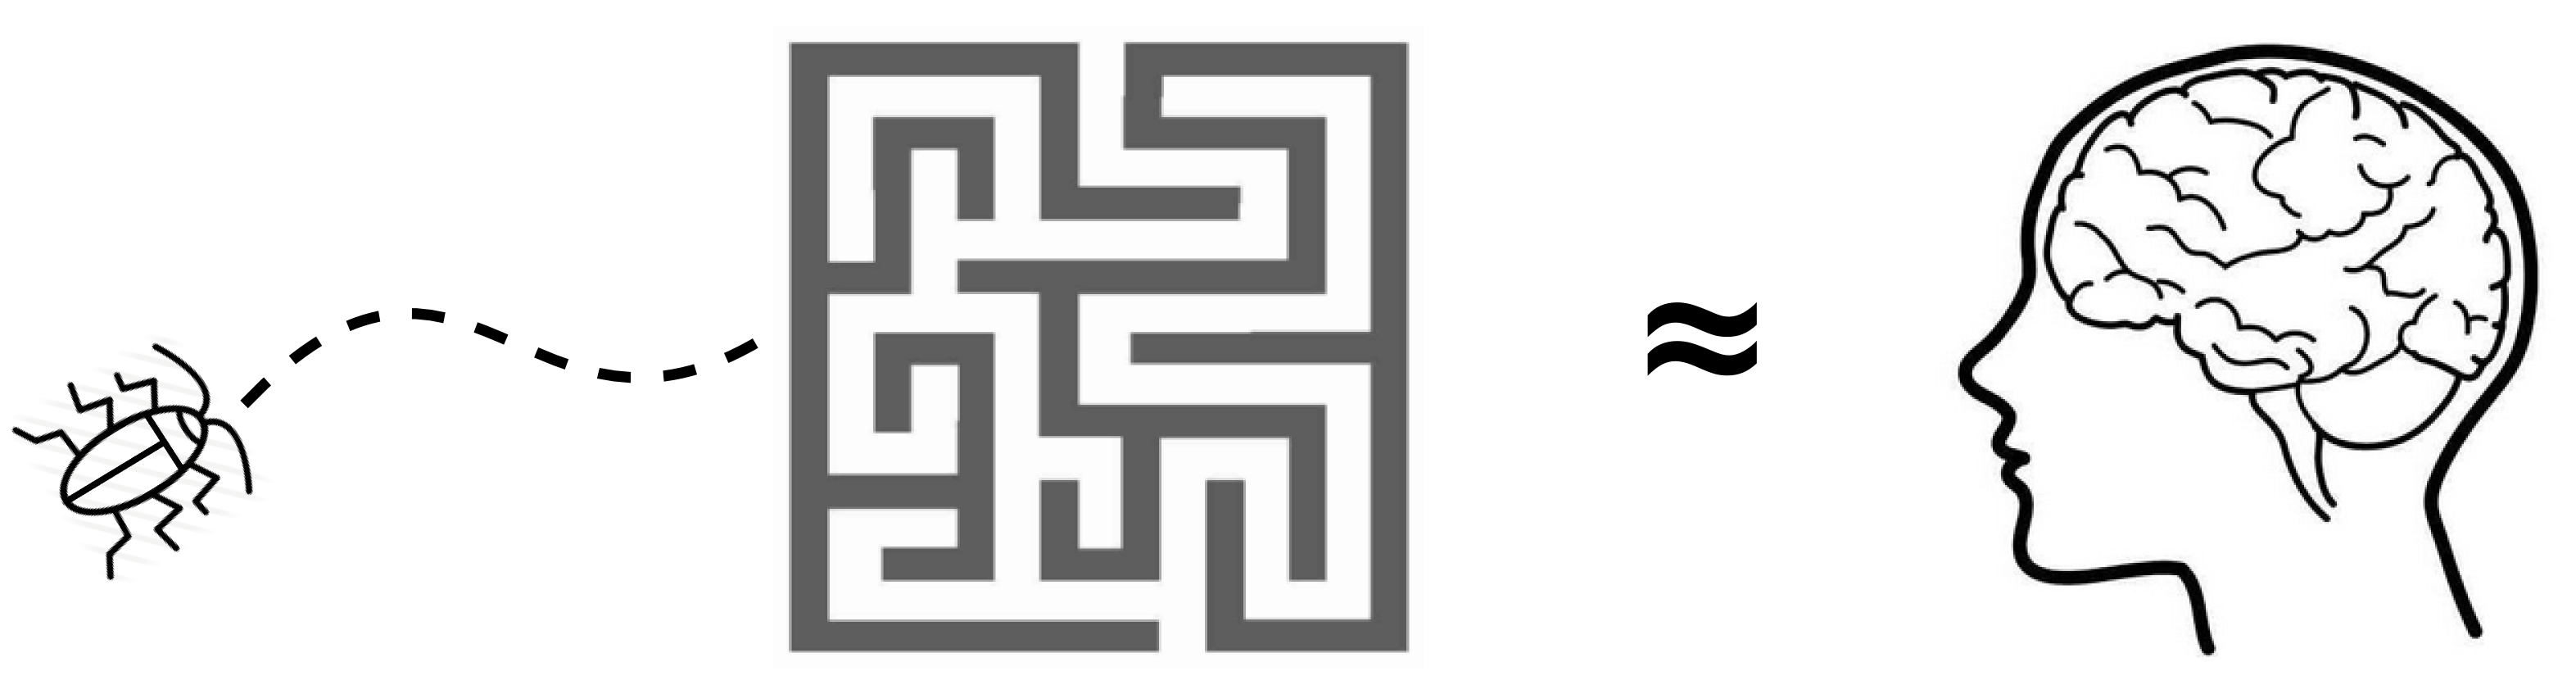
\includegraphics[scale=0.5]{maze-metaphor.png}}}
\end{equation}

The main idea is to regard ``thinking'' as a \emp{dynamical system} operating on \emp{mental states}:
\begin{equation}
\label{fig:mental-state}
\vcenter{\hbox{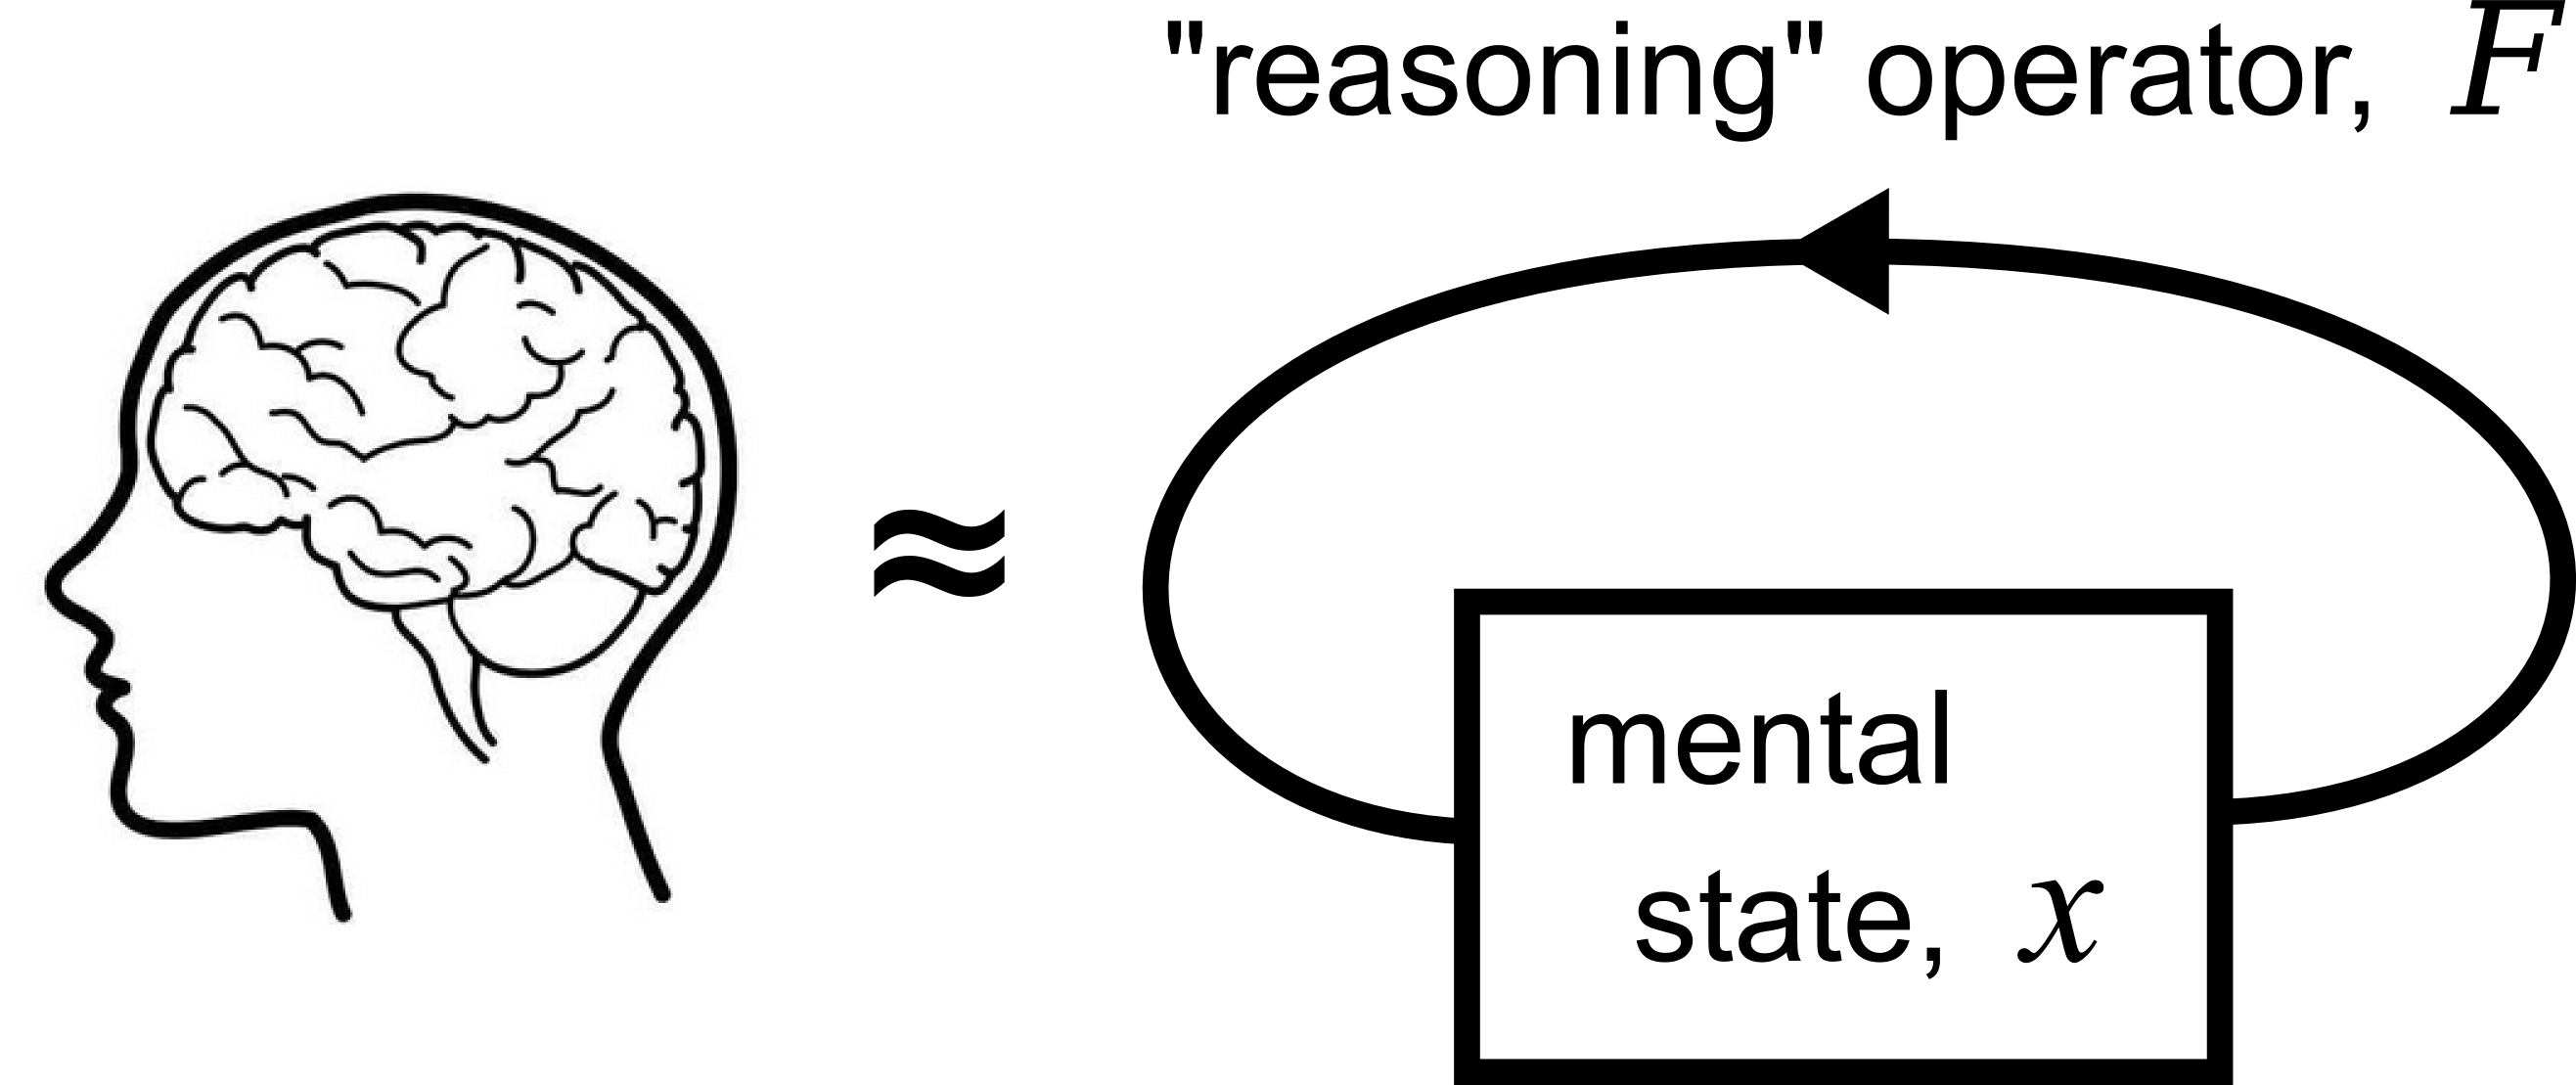
\includegraphics[scale=0.5]{mental-state.png}}}
\end{equation}

For example, a mental state could be the following set of propositions:
\let\labelitemi\labelitemii
\begin{itemize}
\item I am in my room, writing a paper for AGI-17.
\item I am in the midst of writing the sentence, ``I am in my room, ...''
\item I am about to write a gerund phrase ``writing a paper...''
\end{itemize}

Thinking is the process of \emp{transitioning} from one mental state to another.  Even as I am speaking now, I use my mental state to keep track of where I am at within the sentence's syntax, so that I can structure sentences grammatically.

The following 3 theories are actually synonymous:
\begin{itemize}
\item in artificial intelligence, \textbf{reinforcement learning (RL)}
\item in operations research, \textbf{dynamic programming}
\item in modern control theory, the \textbf{state space} description
\end{itemize}

%\begin{itemize}
%\item numerical optimization (eg gradient descent)
%\item differential equations governing time evolution
%\item dynamical systems theory, control theory, dynamic programming, reinforcement learning
% \item Lie algebra and $C^*$-algebra of continuous operators
% \item matrix theory, iteration and fixed-point theory
%\item neural networks and deep learning ... etc.
%\end{itemize}

%=======================================================================================
\begin{comment}

\subsection{Related work}

Google's \textbf{PageRank} is one of the earlier successful applications of vector-space and matrix techniques.  The \textbf{Word2Vec} \cite{Weston2015} algorithm that maps natural-language words to vectors is also spectacularly successful and influential;  it demonstrated the potential advantages of vector representations.  As for reinforcement learning, Q-learning (a form of RL) has been combined with deep learning to successfully play Atari games \cite{Mnih2013};  Their architecture is exactly the same as ours, except that we are trying to refine the internal structure of the learner.
%, both exploit the efficiency of vector and matrix calculus.

This is the cartoon version of our architecture:
\begin{equation}
\vcenter{\hbox{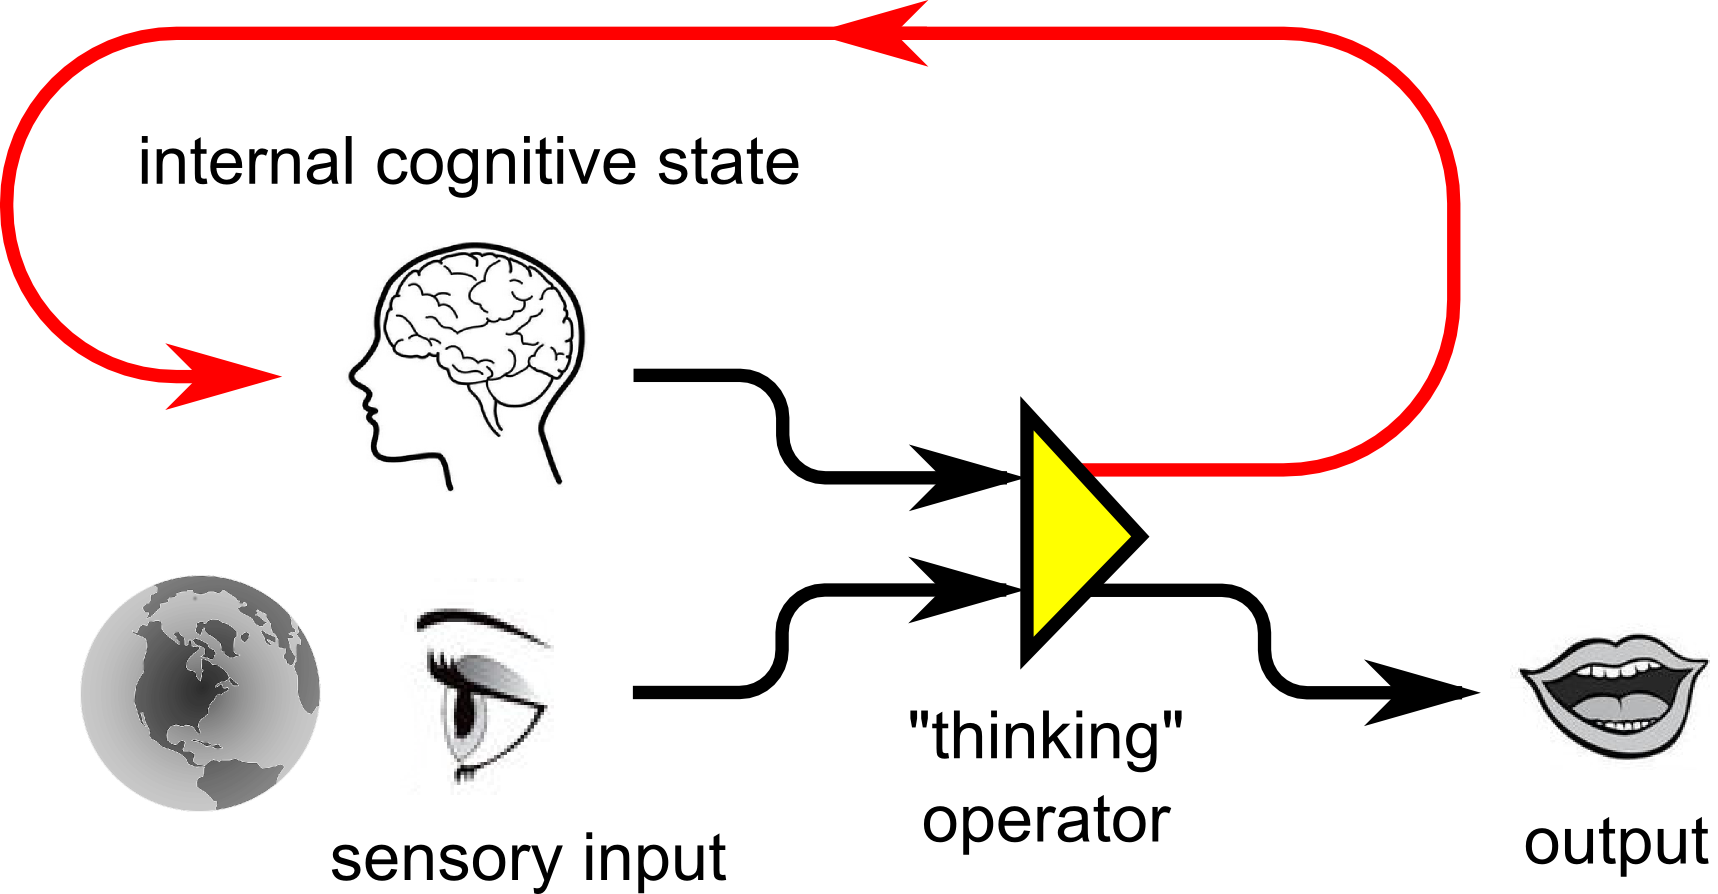
\includegraphics[scale=0.5]{architecture-cartoon.png}}}
\end{equation}

%=======================================================================================
\end{comment}

\section{Control theory / dynamical systems theory}

The cognitive state is a vector $\vect{x} \in \mathbb{X}$ where $\mathbb{X}$ is the space of all possible cognitive states, the reasoning operator $\vect{F}$ is an \textbf{endomorphism} (an \textbf{iterative map}) $\mathbb{X} \rightarrow \mathbb{X}$.

Mathematically this is a \emp{dynamical system} that can be defined by:
\begin{eqnarray}
\boxed{\mbox{discrete time}} \quad \quad & \vect{x}_{t+1} = \vect{F}(\vect{x}_t) \label{eqn0}\\
\boxed{\mbox{continuous time}} \quad \quad & \dot{\vect{x}} = \vect{f}(\vect{x}) \label{eqn1}
\end{eqnarray}
%($\vect{F}$ is implemented as the deep learning network in our approach.)

In our cognitive architecture design, $\vect{F}$ is implemented as a deep neural network (the word ``deep'' simply means ``many layers''):
\begin{equation}
\vcenter{\hbox{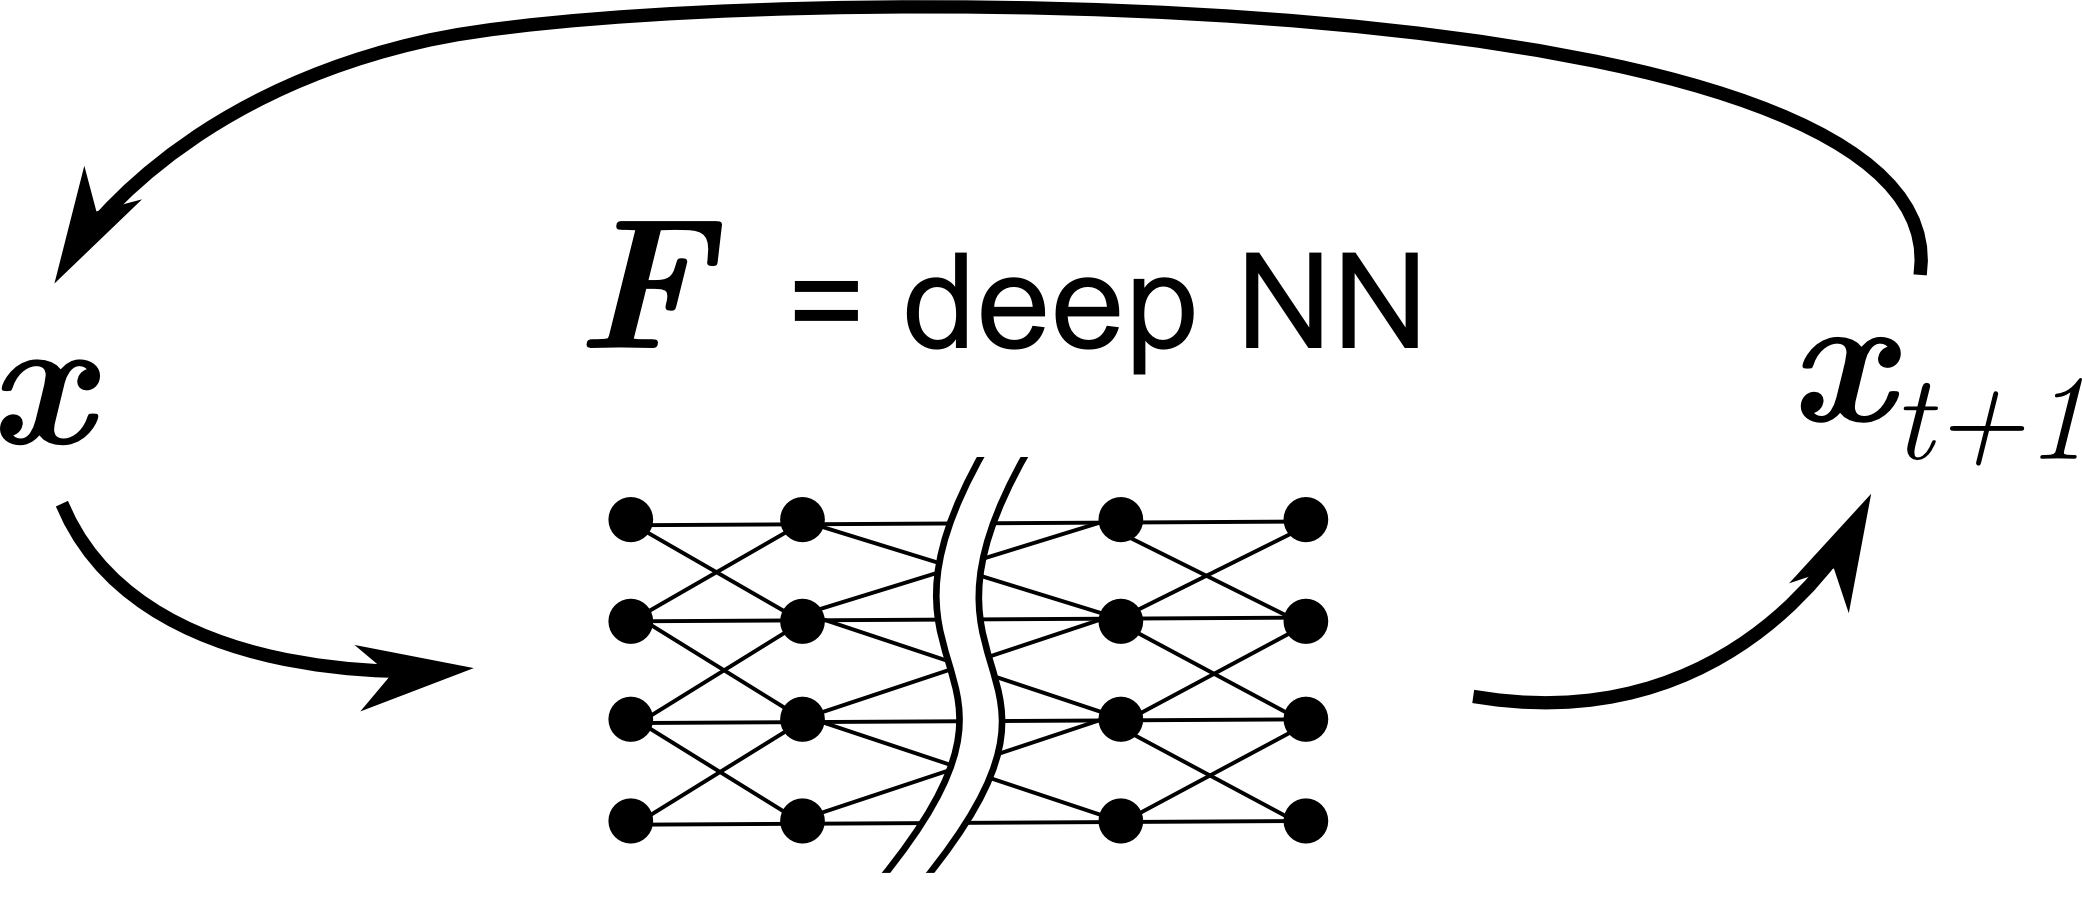
\includegraphics[scale=0.7]{genifer-model-00.png}}}
\end{equation}

A \textbf{neural network} is a non-linear operator with many parameters (called ``weights''):
\begin{eqnarray}
\mbox{\footnotesize each layer's } \tikzmark{ww} \mbox{\footnotesize \textbf{weight} matrix} \quad \quad \mbox{\footnotesize total \# of layers} \tikzmark{LL} \nonumber \\
\nonumber \\
F(\vect{x}) = \sigmoid(W_1 \tikzmark{wa} \sigmoid(W_2 \tikzmark{wb} ... \sigmoid( W_L \tikzmark{wc} \tikzmark{L} \; \vect{x} )))
\begin{tikzpicture}[overlay,remember picture]
  \draw[-, shorten <=26pt, transform canvas={shift={(-10pt,10pt)}}] (ww.center) to (wa.center);
  \draw[-, shorten <=38pt, transform canvas={shift={(-10pt,10pt)}}] (ww.center) to (wb.center);
  \draw[-, shorten <=46pt, transform canvas={shift={(-10pt,10pt)}}] (ww.center) to (wc.center);
  \draw (LL.center) +(-15pt,-3pt) -- ([shift={(-2pt,6pt)}]L.center);
\end{tikzpicture}
\end{eqnarray}
$\sigmoid$ is a sigmoid-shaped non-linear function, applied component-wise to the vectors.

If continuous-time, $\vect{f}$ can also be implemented as neural network, but $\vect{f}$ and $\vect{F}$ are different in nature, they are related by: $\vect{x}(t + 1) = \vect{F}(\vect{x}(t))$.  For ease of discussion, sometimes I mix discrete-time and continuous-time notations.

A \emp{control system} is a dynamical system added with the control vector $\vect{u}(t)$:
\begin{equation}
\dot{\vect{x}}(t) = f(\vect{x}(t), {\color{red} \vect{u}(t)}, t)
\end{equation}
The goal of control theory is to find the optimal $\vect{u}^*(t)$ function, such that the system moves from the initial state $\vect{x}_0$ to the terminal state $\vect{x_\bot}$.

A typical control-theory problem is described by:
\begin{eqnarray}
\boxed{\mbox{state equation}} \quad & \dot{\vect{x}}(t) = \vect{f}[\vect{x}(t), \vect{u}(t), t] \label{eqn1}\\
\boxed{\mbox{boundary condition}} \quad & \vect{x}(t_0) = \vect{x}_0 \,,\, \vect{x}(t_\bot) = \vect{x}_\bot \\
\boxed{\mbox{objective function}} \quad & J = \int_{t_0}^{t_\bot} L[\vect{x}(t), \vect{u}(t), t] dt
\end{eqnarray}
and we seek the optimal control $\vect{u}^*(t)$.

According to control theory, the condition for \textbf{optimal path} is given by the Hamilton-Jacobi equation:
\begin{equation}
\boxed{\mbox{Hamilton-Jacobi equation}} \quad
0 = \frac{\partial J^*}{\partial t} + \min_u H
\end{equation}
%\frac{d}{dt} V(x,t) = \min_u \{ C(x,u) + \langle \nabla V(x,t), f(x,u) \rangle \} 

After the next section I will explain the meaning of $J$, $L$ and $H$.

\section{Reinforcement learning / dynamic programming}

\textbf{Reinforcement learning} is a branch of machine learning that is particularly suitable for controlling an \textbf{autonomous agent} who interacts with an \textbf{environment}.  It uses \textbf{sensory perception} and \textbf{rewards} to continually modify its \textbf{behavior}.  The exemplary image you should invoke in mind is that of a small insect that navigates a maze looking for food and avoiding predators:  $\vcenter{\hbox{
\includegraphics[scale=0.5]{cockroach.png}}}$

A reinforcement learning system consists of a 4-tuple:
\begin{equation}
\boxed{\mbox{reinforcement learning system}} \; = (\vect{x} \in \mbox{States}, \vect{u} \in \mbox{Actions}, R = \mbox{Rewards}, \pi = \mbox{Policy})
\end{equation}
For details readers may see my \textit{Reinforcement learning tutorial} \cite{YanRLtutorialEN}.

%is synonymous with \textbf{dynamic programming}, which is also the main content of modern \textbf{control theory} with the state-space description.

$U$ is the total rewards of a sequence of actions:
%\begin{equation}
%\boxed{\mbox{total value of state 0}} \; U(\vect{x}_0) = \sum_t \; \boxed{\mbox{reward at time t}} \; R(\vect{x}_t, \vect{u}_t)
%\end{equation}
\begin{eqnarray}
\mbox{\footnotesize total value of state 0} \tikzmark{uu} & \quad \quad \quad & \mbox{\footnotesize reward at time $t$} \tikzmark{rr} \nonumber \\
\nonumber \\
\tikzmark{UU} U(\vect{x}_0) & = & \sum_t \; \tikzmark{RR} R(\vect{x}_t, \vect{u}_t)
\begin{tikzpicture}[overlay,remember picture]
  \draw (uu.center) +(-50pt,-3pt) -- ([shift={(4pt,12pt)}]UU.center);
  \draw (rr.center) +(-35pt,-3pt) -- ([shift={(8pt,12pt)}]RR.center);
\end{tikzpicture}
\end{eqnarray}
For example, the value of playing a chess move is not just the immediate reward of that move, but includes the consequences of playing that move (eg, greedily taking a pawn now may lead to checkmate 10 moves later).  Or, faced with delicious food, some people may choose not to eat, for fear of getting fat.

%The goal of \textbf{reinforcement learning} is to learn the \emp{policy function}:
%\begin{equation}
%\begin{tikzcd}[]
%\mbox{policy : ~~state} \arrow[r, mapsto, "\scalebox{0.8}{action}"] & \mbox{state'}
%\end{tikzcd}
%\end{equation}
%when we are given the \emp{state space}, \emp{action space}, and \emp{reward function}:
%\begin{equation}
%\mbox{reward}: \boxed{\mbox{state}} \times \boxed{\mbox{action}} \rightarrow \mathbb{R}
%\end{equation}
%The action $a$ is the same notion as the control variable $u$ in control theory.

The central idea of \textbf{Dynamic programming} is the \textbf{Bellman optimality condition}. Richard Bellman in 1953 proposed this formula, while he was working at RAND corporation, dealing with operations research problems.

The \textbf{Bellman condition} says:  ``\uline{if we cut off a tiny bit from the endpoint of the optimal path, the remaining path is still an optimal path between the new endpoints}.''

\begin{eqnarray}
& \mbox{\footnotesize value of entire path} \tikzmark{uEntire} \quad \quad \mbox{\footnotesize reward of choosing $\vect{u}$ at current state} \tikzmark{rCurrent} \quad \quad \mbox{\footnotesize value of rest of path} \tikzmark{uRest} \nonumber \\
\nonumber \\
& \boxed{\mbox{Bellman equation}} \quad \tikzmark{UEntire} U^*(\vect{x}) = \max\limits_{\vect{u}} \{ \; \tikzmark{RCurrent} R(\vect{u}) + \tikzmark{URest} U^*(\vect{x}_{t+1}) \; \}
\begin{tikzpicture}[overlay,remember picture]
  \draw (uEntire.center) +(-30pt,-3pt) -- ([shift={(4pt,12pt)}]UEntire.center);
  \draw (rCurrent.center) +(-80pt,-3pt) -- ([shift={(4pt,12pt)}]RCurrent.center);
  \draw (uRest.center) +(-65pt,-3pt) -- ([shift={(8pt,12pt)}]URest.center);
\end{tikzpicture}
\end{eqnarray}
This seemingly simple formula is the \uline{entire content} of dynamic programming;  What it means is that:  When seeking the path with the best value, we cut off a bit from the path, thus reducing the problem to a smaller problem;  In other words, it is a \textbf{recursive relation} over time.

In AI reinforcement learning there is an oft-employed trick known as $Q$-learning.  $Q$ value is just a variation of $U$ value;  there is a $U$ value for each state, and $Q$ is the \textbf{decomposition} of $U$ by all the actions available to that state.  In other words, $Q$ is the utility of doing action $\vect{u}$ in state $\vect{x}$.  The relation between $Q$ and $U$ is:
\begin{equation}
U(\vect{x}) = \max\limits_{\vect{u}} \, Q(\vect{x}, \vect{u})
\end{equation}
The advantage of $Q$ is the ease of learning.  We just need to learn the value of actions under each state.  This is so-called ``\textbf{model free learning}''.

%The \emp{Bellman equation} governs reinforcement learning just as in control theory:
%\begin{eqnarray}
%\boxed{\mbox{optimal path}} = & \mbox{choose max reward on current path segment} \nonumber \\
%& \quad + \boxed{\mbox{the rest of optimal path}}
%\end{eqnarray}
%In math notation:
%\begin{equation}
%U^*_t = \max_{u} \{ \; \boxed{\mbox{reward}(u, t)} + U^*_{t-1} \; \}
%\end{equation}
%where $U$ is the ``long-term value'' or \emp{utility} of a path.

%Conceptually, $U$ is the \textbf{integration} of instantaneous rewards over time:
%\begin{equation}
%\boxed{\mbox{utility, or value} U} = \int \boxed{\mbox{reward} R} \,dt
%\end{equation}

\subsection{Internal vs external view of reinforcement learning}

Traditionally, RL deals with acting in an \textit{external} environment; value / utility is assigned to \textit{external} states.  In this view, the \textit{internal} mental state of the agent may change without any noticeable change externally:
\begin{equation}
\vcenter{\hbox{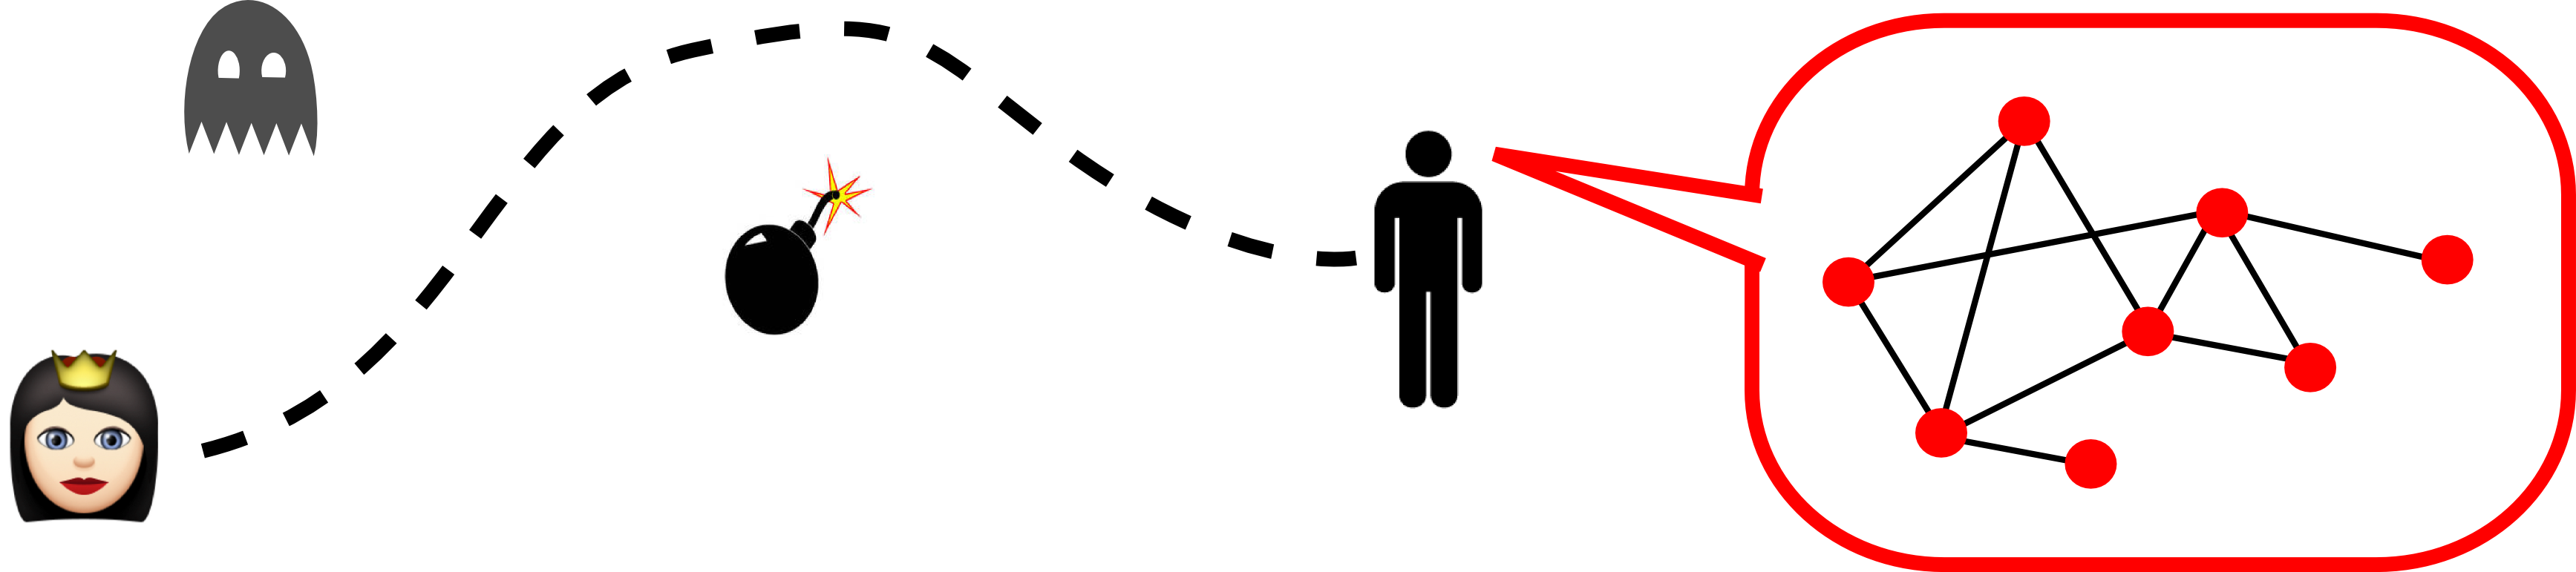
\includegraphics[scale=0.6]{save-princess.png}}}
\end{equation}
The usefulness of RL (ie, the Bellman update technique) makes me wonder if it'd be advantageous to invert the perspective to consider the internal mental landscape instead.  Then, an internal state would have higher utility when it has been visited by many successful ``thinking'' trajectories.

\subsection{Actions = cognitive state-transitions = ``thinking''}

In our system there are 2 things that need to be learned:
\begin{enumerate}
\item The transition function $\vect{F}: \vect{x} \mapsto \vect{x}'$.  $\vect{F}$ represents the \textbf{knowledge} that constrains thinking.  In other words, the learning of $\vect{F}$ is the learning of ``static'' knowledge.
\item Find the optimal trajectory of the state $\vect{x}$.  This corresponds to optimal ``thinking'' under the constraints of static knowledge.
\end{enumerate}
\begin{equation}
\vcenter{\hbox{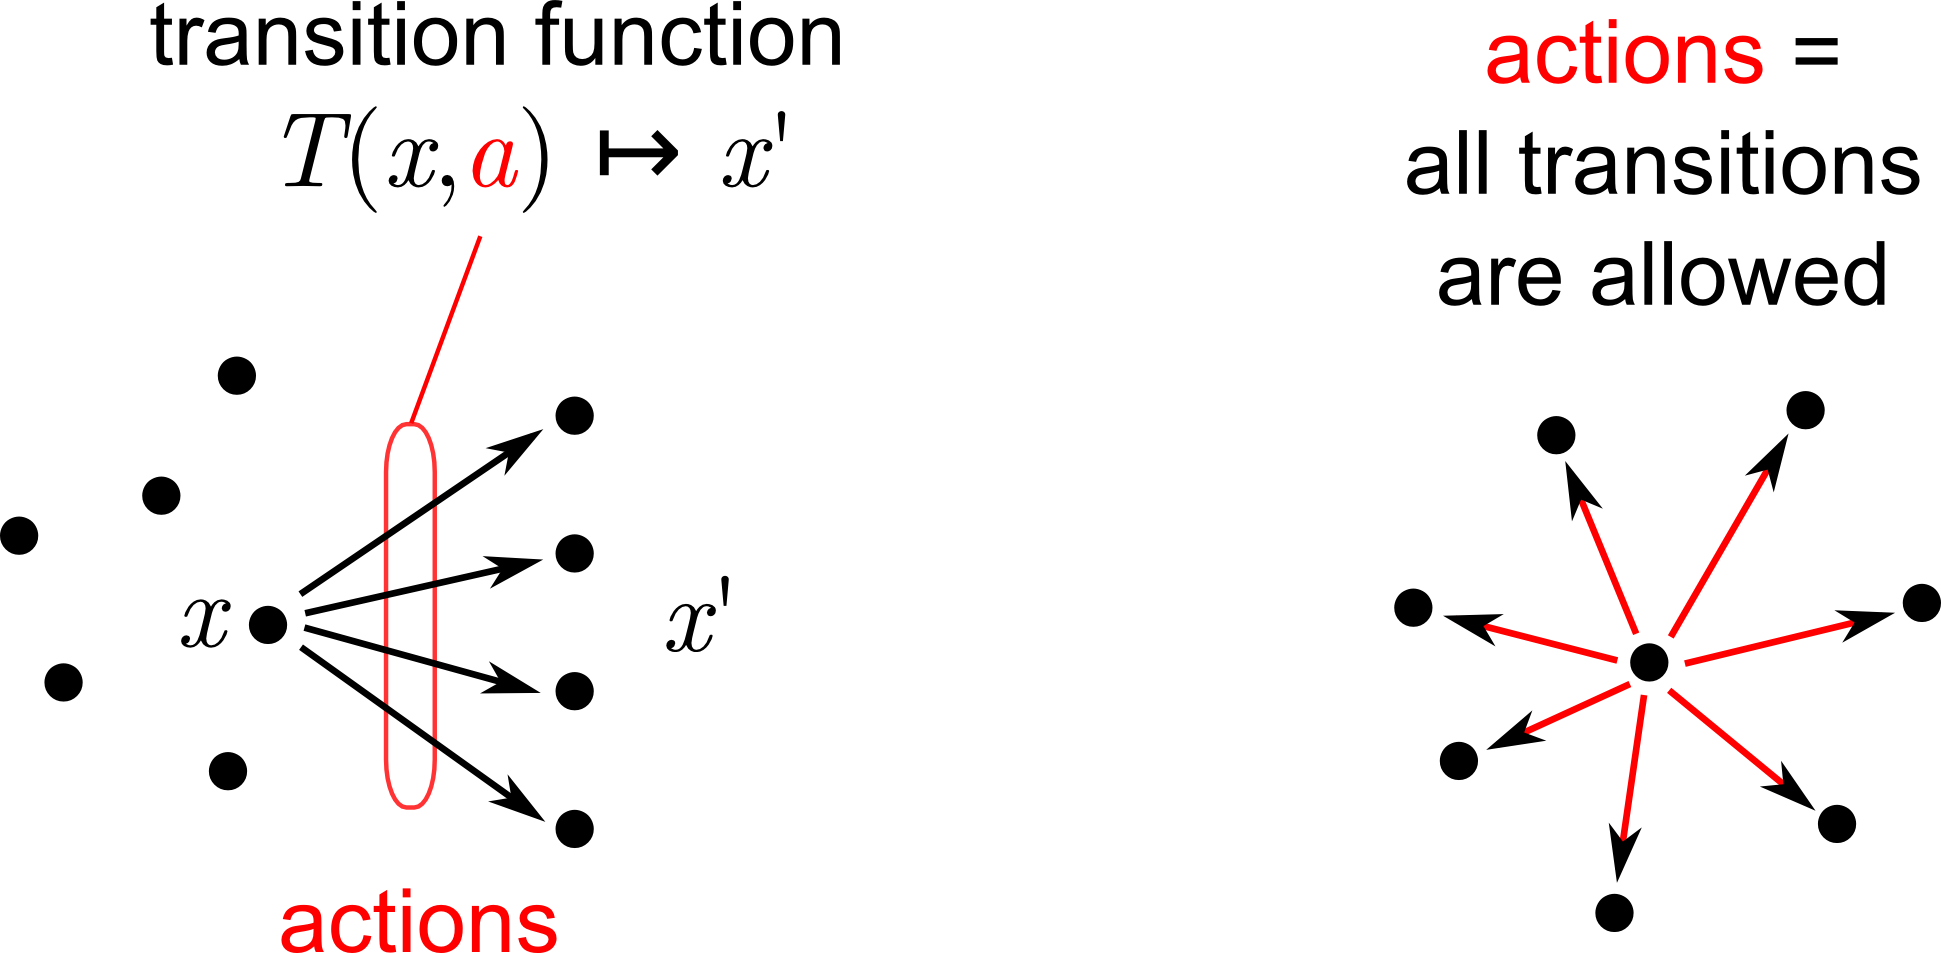
\includegraphics[scale=0.7]{Q-learning-2-views.png}}}
\end{equation}
In traditional reinforcement learning (left view), the system chooses an action $\vect{a}$, and the transition function $\vect{F}$ gives the probability of reaching each state $\vect{x}_i$ given action $\vect{a}$.  In our model (right view), all possible cognitive states are potentially \textbf{reachable} from any other state, and therefore the action $a$ coincides with the next state $x'$.

\begin{comment}
%==================================================================================
Under the reinforcement learning framework, intelligence is decomposed into \textbf{thinking} and \textbf{learning}:
\begin{itemize}
\item \emp{Thinking} means finding the optimal trajectory of $\vect{x}$ according to the \textbf{knowledge} stored in the deep NN.  This is achieved using the Bellman equation to calculate $\vect{u}^*$.  The trajectory of $\vect{x}$ is constrained by the deep NN (in other words, the system must think in accordance with \textbf{correct knowledge}).  While thinking, the deep NN stays \textbf{constant}.

\item \emp{Learning} means learning the weights in the deep NN.  Changing $W$ changes $\vect{F}$, which determines the state equation (\ref{eqn0}), so the entire system becomes a new one.  In other words, deep NN learning is a kind of \textbf{second-order learning}:  Consider 2 systems $\vect{F}$ and $\vect{F} + \epsilon \hat{\vect{F}}$, after \uline{many trials} of thinking with different premises, if the average reward is higher in the altered system, $\vect{F}$ will learn towards the $\hat{\vect{F}}$ direction.
% 即是根据已学得的\textbf{知识}(知识储存在 deep NN 里),在思维空间中找寻 $\vect{x}$ 最优的轨迹,方法是根据 Bellman 方程计算 $\vect{u}^*$。 $\vect{x}$ 的轨迹受 deep NN 约束(亦即是说,系统只能依据\textbf{正确的知识}去思考),思考时 deep NN 是\textbf{不变}的。
%\item \emp{学习}就是学习神经网络 deep NN 的 weights $W_\ell$,改变 $W$ 即改变 $\vect{F}$,而$\vect{F}$ 决定\textbf{状态方程} (\ref{eqn0}),所以整个系统变了另一个系统。 换句话说,deep NN 的学习是一种 \textbf{second-order learning}: 考虑两个系统 $\vect{F}$ 和 $\vect{F} + \epsilon \hat{\vect{F}}$,经过很多次思考过程,如果奖励的平均值在后者有所增加,则 $\vect{F}$ 向 $\hat{\vect{F}}$ 方向学习。
\end{itemize}
%==================================================================================
\end{comment}

\subsection{Prior art}

The minimalist architecture based on reinforcement learning has been proposed by Itimar Ariel from Israel, in 2012 \cite{Arel2012}, and I also independently proposed in 2016 (precursor of this paper).  The prestigious researcher of signal processing, Simon Haykin, recently also used the ``RL + memory'' design, cf. his 2012 book \textit{Cognitive dynamic systems} \cite{Haykin2012}. Vladimir Anashin in the 1990's also proposed this kind of cognitive architecture \cite{Anashin2009}.  There may exist more precedents, eg: \cite{Ivancevic2006}.

\subsubsection{Comparison with AIXI}

AIXI's environmental setting is the same as ours, but its agent's internal model is a universal Turing machine, and the optimal action is chosen by maximizing potential rewards over all programs of the UTM.  In our (minimal) model, the UTM is \uline{restricted} to an RNN, where the RNN's \textbf{state} is analogous to the UTM's \textbf{tape}, and the optimal weights (program) are found via Bellman optimality.

\begin{tcolorbox}[colback=grey, breakable, enhanced]
\subsection*{Connections with the Hamiltonian}

In \emp{reinforcement learning}, we are concerned with two quantities:
\let\labelitemi\labelitemii
\begin{itemize}
\item $R(\vect{x}, \vect{u})$ = \emp{reward} of doing action $\vect{u}$ in state $\vect{x}$
\item $U(\vect{x})$ = \emp{utility} or \emp{value} of state $\vect{x}$ 
\end{itemize}
Simply put, \textbf{utility} is the integral of instantaneous \textbf{rewards} over time:
\begin{equation}
\boxed{\mbox{utility} $U$} = \int \boxed{\mbox{reward} $R$} \,dt
\end{equation}
%(价值有时用 $V$ 表示,但为避免和势能 $V$ 混淆故不用。)

In \emp{control-theoretic} parlance, it is usually defined the \textbf{cost functional}:
\begin{equation}
\boxed{\mbox{cost } $J$} = \int L dt + \Phi(\vect{x}_\bot)
\end{equation}
where $L$ is the \textbf{running cost}, ie, the cost of making each step; $\Phi$ is the \textbf{terminal cost}, ie, the value when the terminal state $\vect{x}_\bot$ is reached.

%Define a continuous version of ``utility'':
%\begin{equation}
%V(x,t) = \min_u \{ \int_t^{t_\bot} C(x,u)dt + \Phi(x_\bot,t_\bot) \} 
%\end{equation}
%where $t$ is time, $u$ is a set of control parameters, $C$ is the \emp{cost-rate} function:
%\begin{equation}
%\int C dt = R = \mbox{reward}
%\end{equation}
%This integral expresses the ``cost of the path'', whereas $\Phi(x_\bot,t_\bot)$ is the ``cost at termination''.

In \emp{analytical mechanics} $L$ is known as the \textbf{Lagrangian}, and the time-integral of $L$ is called the \textbf{action}:
\begin{equation}
\boxed{\mbox{action } $S$} = \int L dt
\end{equation}
Hamilton's \emp{principle of least action} says that $S$ always takes the \textbf{stationary value}, ie, the $S$ value is extremal compared with neighboring trajectories.

The \textbf{Hamiltonian} is defined as $\displaystyle H = L + \frac{\partial J^*}{\partial \vect{x}} \vect{f}$, which came from the method of \textbf{Lagrange multipliers}.  For details please refer to my \textit{Control theory tutorial}\cite{YanControlTheoryTutorial}.

All these are the same thing, so there is this correspondence:
\begin{equation}
\begin{tabular}{|c|c|c|}
\hline 
\emp{Reinforcement learning} & \emp{Control theory} & \emp{Analytical mechanics} \\ 
\hline
utility or value $U$ & cost $J$ & action $S$ \\ 
\hline 
instantaneous reward $R$ & running cost & Lagrangian $L$ \\ 
\hline 
action $a$ & control $u$ & (external force?) \\
\hline
\end{tabular} 
\end{equation}

%用比较浅显的例子: 和美女做爱能带来即时的快感 (= 奖励 $R$),但如果强奸的话会坐牢,之后很长时间很苦闷,所以这个做法的长远价值 $U$ 比其他做法较低,正常人不会选择它。

Interestingly, the reward $R$ corresponds to the \textbf{Lagrangian} in physics, whose unit is ``energy'';  In other words, ``desires'' or ``happiness'' appear to be measured by units of ``energy'', this coincides with the idea of ``positive energy'' in pop psychology.  Whereas, long-term value is measured in units of $[\mbox{energy} \times \mbox{time}]$.

%一个智能系统,它有「智慧」的条件,就是每时每刻都不断追求「开心能量」或奖励 $R$ 的最大值,但它必需权衡轻重,有计划地找到长远的效用 $U$ 的最大值。

This correspondence of these 3 theories is explained in detail in Daniel Liberzon's book \cite{Liberzon2012}.  While this correspondence has very interesting philosophical implications, it may not be very useful in practice:  the traditional AI system is discrete-time; converting it to continuous-time seems to increase the computational burden.  The recent advent of \textbf{symplectic integrators} \cite{} are known to produce better numerical solutions that retain qualitative features of the exact solution, eg. quasi-periodicity.

\begin{comment}
%==================================================================================
An interesting insight from control theory is that our system is a Hamiltonian dynamical system in a broad sense.

Hamilton's \emp{principle of least action} says that the trajectories of dynamical systems occuring in nature always choose to have their action $S$ taking \textbf{stationary values} when compared to neighboring paths.  The action is the time integral of the Lagrangian $L$:
\begin{equation}
\boxed{\mbox{Action} S} = \int \boxed{\mbox{Lagrangian} L} \; dt
\end{equation}
From this we see that the Lagrangian corresponds to the instantaneous ``rewards'' of our system.  It is perhaps not a coincidence that the Lagrangian has units of \textbf{energy}, in accordance with the folk psychology notion of ``positive energy'' when we talk about desirable things.

The \emp{Hamiltonian} $H$ arises when we consider a typical control theory problem;  The system is defined via:
\begin{eqnarray}
\mbox{state equation:} \quad & \dot{\vect{x}}(t) = \vect{f}[\vect{x}(t), \vect{u}(t), t] \\
\mbox{boundary condition:} \quad & \vect{x}(t_0) = \vect{x}_0 \,,\, \vect{x}(t_\bot) = \vect{x}_\bot \\
\mbox{objective function:} \quad & J = \int_{t_0}^{t_\bot} L[\vect{x}(t), \vect{u}(t), t] dt
\end{eqnarray}
The goal is to find the optimal control $\vect{u}^*(t)$.

Now apply the technique of \emp{Lagrange multipliers} for finding the maximum of a function, this leads to the new objective function:
\begin{equation}
U = \int_{t_0}^{t_\bot} \{ L + \vect{\lambda}^T(t) \left[ f(\vect{x}, \vect{u}, t) - \dot{\vect{x}} \right] \} dt
\end{equation}
So we can introduce a new scalar function $H$, ie the Hamiltonian:
\begin{equation}
H(\vect{x}, \vect{u}, t) = L(\vect{x}, \vect{u}, t) + \vect{\lambda}^T(t) f(\vect{x}, \vect{u}, t)
\end{equation}
Physically, the unit of $\vect{f}$ is velocity, while the unit of $L$ is energy, therefore $\vect{\lambda}$ should have the unit of \emp{momentum}.  This is the reason why the phase space is made up of the diad of $(\mbox{position}, \mbox{momentum})$.

%==================================================================================
\end{comment}

The equation of motion for the continuous-time case is the famed \emp{Hamilton-Jacobi-Bellman equation}:
% \footnote{To digress a bit, this equation is also analogous to the \emp{Schr\"{o}dinger equation} in quantum mechanics:
%\begin{equation}
%i \hbar \frac{\partial}{\partial t} \Psi(x,t) = \left[ V(x,t) + \frac{-\hbar^2}{2\mu} \nabla^2 \right] \Psi(x,t).
%\end{equation}
%where $\Psi$ is analogous to our $U$ (perhaps $\Psi$ is something that nature wants to optimize?)}
\begin{equation}
\boxed{\mbox{Hamilton-Jacobi-Bellman}} \quad
0 = \frac{\partial U^*}{\partial t} + \min_u H
\end{equation}
of which the \emp{Schr\"{o}dinger equation} is a special case.

%All these ``physical'' ideas flow automatically from our definition of \textbf{rewards}, without the need to introduce them artificially.  But these ideas seem not immediately useful to our project, unless we are to explore \textbf{continuous-time} models.

\end{tcolorbox}

\section{Future directions}

\begin{itemize}
\item \textbf{Relation to logic-based AI:}  In the system's state equation (\ref{eqn0}), $\vect{F}$ is free to change ($\vect{F}$ represents learned knowledge).  In other words, the entire system almost has no structure.  Searching for a candidate $\vect{F}$ in the infinite-dimensional function space is impractical, so we need to introduce the structure of logic-based AI into this system, such that the search space for $\vect{F}$ is reduced.  In machine learning, this is known as \textbf{inductive bias}, the \textit{sine qua non} of speeding up learning.  This will be addressed in our 2nd paper \textit{A bridge between logic and neural} \cite{YanBridge}.

\item \textbf{Memory:}  In this minimal architecture there is no episodic memory, this will be dealt with by our 3rd paper, \textit{The structure of memory} \cite{YanMemory}.

\end{itemize}

\begin{comment}
%==================================================================================
\section{Deep learning}

The combination of deep learning with reinforcement learning, ie deep reinforcement learning (DRL), is very powerful.  For example, DRL is able to play Atari games to human levels \cite{Mnih2013}.  Their architecture is depicted in this diagram:
\begin{equation}
\vcenter{\hbox{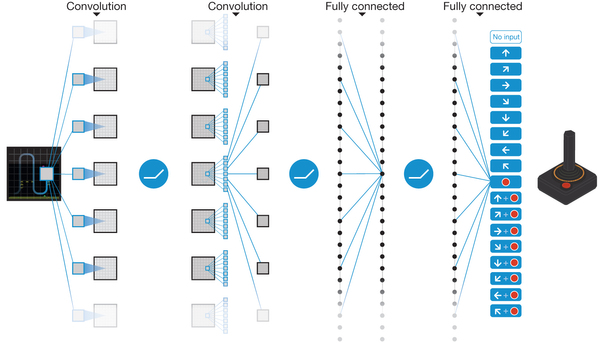
\includegraphics[scale=0.5]{Atari-Q-learning.jpg}}}
\end{equation}

Recall our main architecture:
\begin{equation}
\vcenter{\hbox{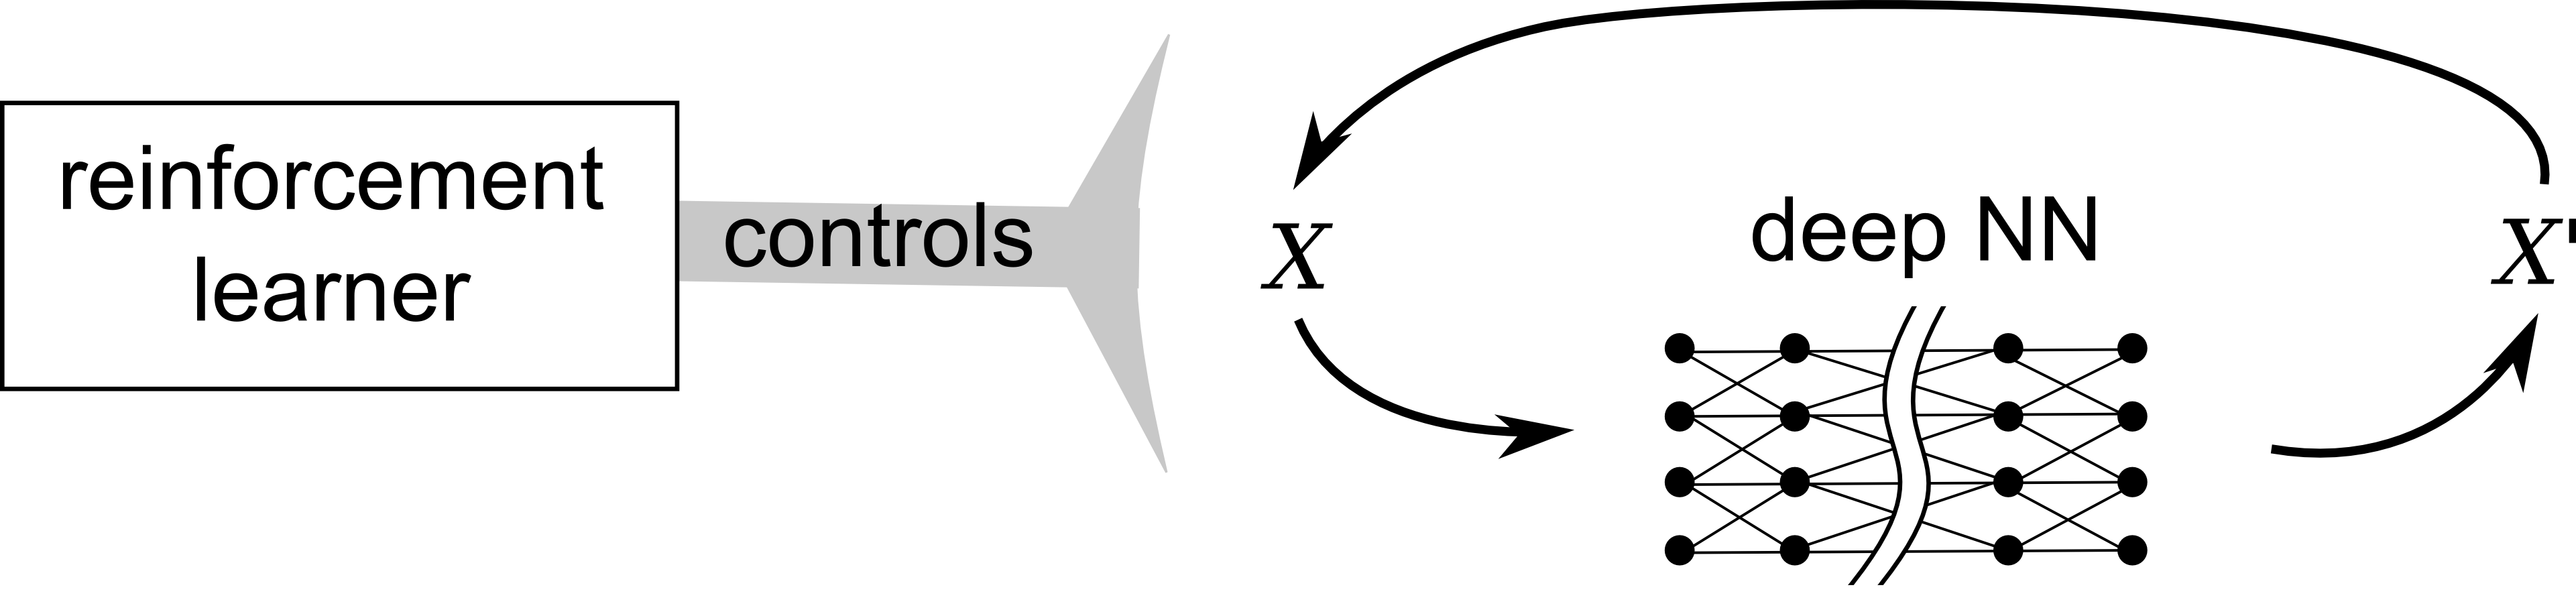
\includegraphics[scale=0.5]{genifer-model-0.png}}}
\end{equation}

The ``transition function'' neural network can also take an \textbf{action} parameter $u$:
\begin{equation}
\vcenter{\hbox{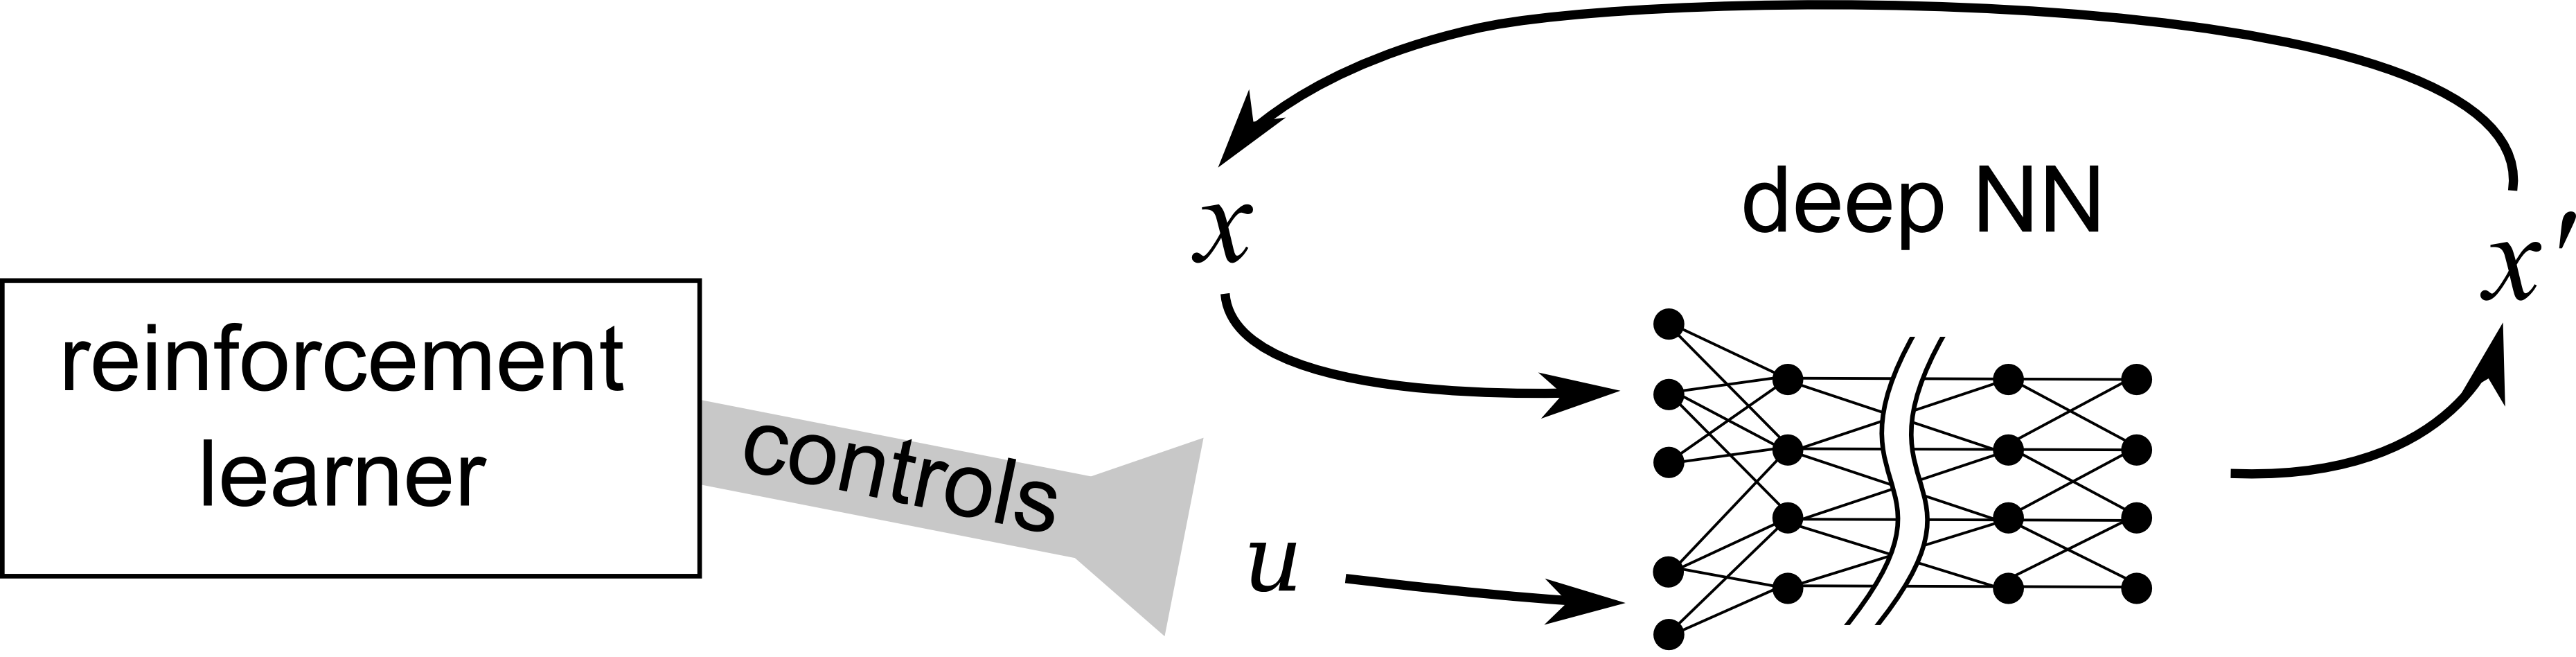
\includegraphics[scale=0.5]{model-with-u.png}}}
\end{equation}
But such a neural network requires a novel learning algorithm that is \textbf{reward-driven} rather than the traditionally \textbf{error-driven} back-propagation.  Such an algorithm is difficult to design because it cannot rely on old-fashioned gradient descent.

One solution that avoids the difficulty is to make the neural network compute the Q-value:
\begin{equation}
\vcenter{\hbox{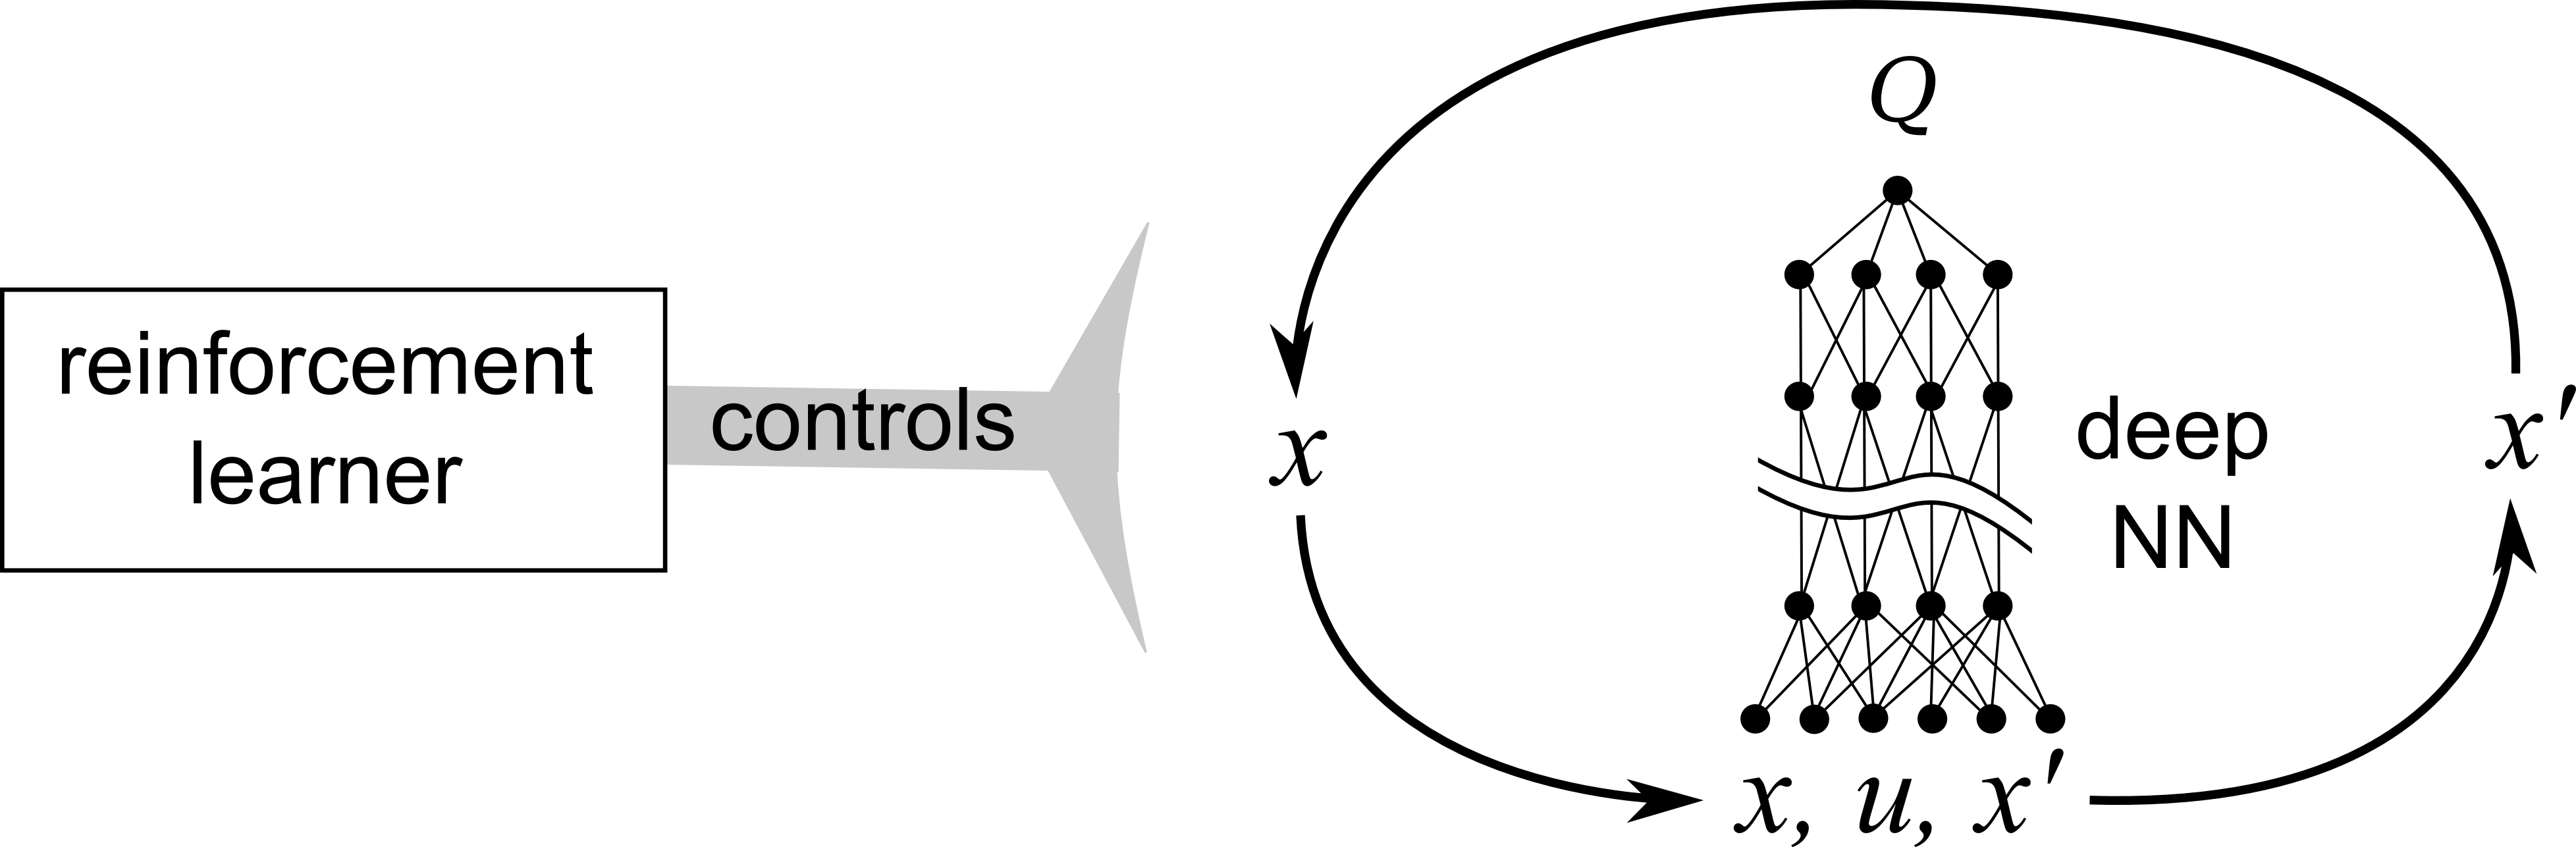
\includegraphics[scale=0.5]{model-Sayaka.png}}}
\end{equation}
This means that we can compute $Q$ for any transition $x \stackrel{u}{\mapsto} x'$.  During the ``action'' (ie, ``thinking'') stage, we hold $x$ fixed, and search for $(u, x')$ that maximizes $Q$;  This can be done by \textbf{stochastic gradient descent}.  During the ``learning'' stage, we are given certain transitions $(x, u, x')$ and we train the neural network to adjust $Q$ via standard \textbf{Bellman update}.

%==================================================================================
\end{comment}

% ================================== comment out ==================================
\iffalse

From the viewpoint of reinforcement learning, we aim to learn the \emp{policy} function: \par
\begin{equation}
\begin{tikzcd}[]
\mbox{policy : ~~state} \arrow[r, mapsto, "\scalebox{0.8}{action}"] & \mbox{state'}
\end{tikzcd}
\end{equation}
Where $K$ can be regarded as the \emp{mental state}, and thus an \emp{action} in RL turns $K$ into $K'$.

In our system, there are 2 pathways that act on $K$, via RNN and RL respectively: \par
\begin{equation}
\begin{tikzcd}[column sep=huge]
& K'_1 \arrow[dd, dashed, no head, "\scalebox{1.3}{$\approx$}"] \\
K \arrow[ur, "\mbox{RL}"] \arrow[dr, "\mbox{RNN}"'] & \\
& K'_2
\end{tikzcd}
\end{equation}
In RL, the action $a$ acts on $K$, whereas in RNN, $R$ acts on $K$.

\emp{Note}: RNN and RL are learning algorithms, and if they are both applied to the same problem, conflicts will necessarily arise, unless there is a way to combine them.

At state $K$, we estimate the Q-value $Q(K \stackrel{a}{\mapsto} K')$.  The action that would be chosen at state $K$ is $\displaystyle \arg\max_a Q(K \stackrel{a}{\mapsto} K')$.  This could be used to train the RNN via $\displaystyle K \vdash_W ...^n K'$.

RL 在众多状态 $K$ 之间游荡,学习 $Q(K \mapsto K')$。  因为 RL 独有奖励讯息,我们必需用 RL 来教导 RNN 学习,反之不可。  第一个问题是: RL 如何在 $K$ 之间游荡?   游荡是随机的,但也可以借助 RNN 的随机性、或在 RNN 自身的游荡中注入更多随机性、或者根本就是 RL 自己产生的随机性。  接下来的问题是: RNN 如何用 $Q$ 值来诱发学习?

RNN 的 ``$n$-fold'' 学习可以通过以下方式实现: 
\begin{itemize}
\item stochastic forward-backward propagation
\item genetic?
\item 最有趣的是 Hebbian learning,因为它似乎特别适合这情况。  
\end{itemize}

RNN 的本质是什么?  它似乎是一个 recurrent hetero-associative memory。  但其实它还需要将 input 作类似於 Word2vec 的 encoding。  这个 encoding 将「相似」的思维状态 $K$ 归到同类。  利用空间中的相似度,RL 可以用一些连续函数来近似 Q 值(详细情况还有待分析)。

另一个问题是: 虽然用函数的近似可以做到 generalization,但另一个方法是利用状态 $K$ 中的空位作暂时储存。 这两者似乎很不同。  问题似乎在於: 状态转换 $K \mapsto K'$ 是不是对应於逻辑中的\emp{一条} rule?  答案似乎是 yes。  这个共识是很重要的。  如果用 decision tree,需要的是向量空间中的相似度。

现在的关键是「状态变量」。  因为它可以做到符号逻辑中靠变量的 generalization,这是前所未有的。  这种 generalization 似乎不需要相似度,因为它是符号的!  会不会在向量空间中的状态变量 能够做到之前逻辑变量做不到的动作?  不管怎样,用 RNN 学习这些变量的动作似乎是很难的,因为这些动作似乎不是对\emp{误差}的梯度下降。  除非这些动作本身也近似於其他动作,但那是怎样的近似?  学习 multi-step logic 其实和以前的 forward / backward chaining 没有分别!  唯一分别是命题的 representation 改变了,它未必像符号的 concatenation。  所以问题仍然是 ``$n$-fold'' 学习法。 

而且注意: RL 的 generalization 根本上不同於 rules 空间中的 generalization。 前者是思维空间 $K$ 中的一般化,后者也可以是 $K$ 空间的一般化,但也可以是依赖「状态变量」的一般化。

一般来说,RL 和 RNN 的行动和学习,是可以互相独立的。  

还有 heterarchical 的分类法。  想用 decision tree 或什么,达到不同网络的\emp{分工}。  在组织知识这方面,深度网络有没有用?  可以想像,在视觉识别中,在网络的最上层有很多 objects,而它们都可以还原到底层的 features。  网络有更多层,可以识别的事物更抽象。  但现在我们要的不是\emp{模式识别},而是 mapping。 特别是抽象模式的 mapping。  想要的是: 大量的 rules,将不同的 $K$ 映射到新的 $K'$。

还有一点要澄清的是: 究竟每一个「思元素」在向量空间中是不是\emp{一点}?  如果有了这个「思元素 = 点」假设,则每次 iteration 应该会删除一个思元素,而用另一个(全新的)思元素取代之。  这样,$K \mapsto K'$ mapping 就有了更确定的结构。  这样的 setup 已经很接近 logic 系统,但其学习算法仍然很有 combinatorial 的 ``feel''。 (因为只有当两个 rules 串连之后,才能达到某个结论,而这个串连有没有中间的 continuous 状态?)  这种串连通常是怎样找到的?  

现在有一转机: 如果「思元素 = 点」,则「状态变量」的形成似乎会很普遍,而我们可以集中研究如何学习 single-step rules。 RL 的 rewards 可以指导学习,但这些「终极 rewards」对学习的细节没有指导作用。  我们似乎可以用「\emp{时间延迟}」来达到「状态变量」的效果,这个做法无形中增加了使用状态变量的机会。  

现在总结一下仍然有待回答的问题:
\begin{itemize}
\item RL 的 generalization 如何做?
\item iterative thinking map 如何 learn?
\item 
\end{itemize}

Hebbian 的情况是: 有某一 I/O pattern; 我想 strengthen 这 pattern。 

Assuming the learning is correct, $K'_1$ and $K'_2$ should be roughly the same \textemdash~ but this ignored the possibility that one path may take multiple steps to converge with the other path.  \footnote{This situation has been encountered in term rewriting systems (TRS):  If in a TRS any 2 different rewriting paths always converge to the same result, it is said to have the \emp{Church-Rosser property}.  For example the $\lambda$-calculus invented by Church has this property.} 

Now I stipulate that $R$ be more ``refined'', that is to say, applying $D^n$ times may be equivalent to applying $a$ once:
\begin{equation}
\begin{tikzcd}[column sep=huge]
& K'_1 \arrow[dd, dashed, no head, "\scalebox{1.3}{$\approx$}"] \\
K \arrow[ur, "\scalebox{1.3}{$a$}"] \arrow[dr, "{\scalebox{1.3}{$D^n$}}"'] & \\
& K'_2
\end{tikzcd}
\end{equation}
Using a different notation, $a$ is the \emp{restriction} or \emp{section} of $D^n$ at point $K$: $a = D^n|_K$.

Now the question is, do the RNN and RL paths have any \textit{essential} difference?
\begin{itemize}
\item Their internal \emp{representations} are different:\par
\dashh RNN is a multi-layer neural network\par
\dashh RL's representation is $Q(\mbox{state},\mbox{action})$, usually stored as a \textit{look-up table}, although $Q$ could be approximated by a neural network as well.
\item RL learns through \emp{rewards}, RNN learns from \emp{errors}.  Thus RL has broader applicability, because not all questions have ``correct answers'' that could be measured by errors.  In RL we just need to praise Genifer whenever she displays good behavior.
\item The internal cognitive state $K$ exists because of RNN:  it is simply the vector input and output of the RNN.  Without this $K$, RL would be clueless as to what are its internal states.  It can be said that the RNN provides a \textit{machinery} for RL to control.
\end{itemize}

% programming needed:
% RNN: with special back-prop
% RL: approximate Q(K,a), using special NN that can find max also

% 整体来说,RL 可以操控的 actions 包括:
% \begin{enumerate}[\tab (A)]
% \item apply $K \stackrel{D}{\mapsto} K'$ \par
% 但注意: $K$ 是认知状态,$R$ 是对 $K$ 进行「合乎逻辑的推论」。 所以,无论发生什么事,我们都会将 $R$ 作用在 $K$ 上几次。 换句话说,$R$ 是\ds{必然}进行的动作,或者可以看成是在\ds{背景}下进行的运作,所以不需要用 RL 学习。 %RL 的用处是学习如何在很多 actions 之间选择最好的一个,所以 $R$ 不是 RL 需要学习的 action,它只是。

% \item 改写认知状态 $K \mapsto K'$ \par
% RL 的 actions (A) 是
% 在思考过程中改变 $K$ 的值。 例如我们得到一个局部结论,这个局部结论的状态不是最终答案,但也比什么都没有的效用更高。 改写 $K$ 的方法可以是: 例如 将 $K \mbox{ += } \delta K$,或者 「if $K \in$ 某 region,then $K \mbox{ += } \delta K $」。

% \item 学习: change $R$ \par

From the perspective of reinforcement learning, we could reward some results of multi-step inference: \par
\begin{equation}
\begin{tikzcd}[row sep=tiny]
K_0 \arrow[r, mapsto, "\scalebox{1.3}{$a$}"] & K_\vdash \quad \updownarrow \bigstar
\end{tikzcd}
\end{equation}
$\updownarrow \bigstar$ means ``to give positive or negative rewards''.  We want to learn $a$ which is the action to be taken at state $K$.  The learning algorithm is based on the famous \emp{Bellman optimality condition} (see next section).

Perhaps we should use RL to \textit{guide} the learning in RNN, as RNN is more fine-grained....

To combine the 2 learning approaches, we could use the technique of \emp{interleaving}: for each step apply RL once, apply RNN $n$ times.

% 但 $R$ 本身是 RNN,它还可以透过 back-prop 进行学习,两者似乎是不同的。  Back-prop 是透过 $\frac{\partial}{\partial D}(\mbox{error})$ 的梯度来学习。

The learning in RNN may also involve \emp{neurogenesis} (adding new neurons and connections), but I have not considered this aspect yet.

% RNN 的 $R$ 也是将 $K$ 变成 $K'$ 的作用:\par
%\begin{figure}[h]
%\centering
%\begin{tikzcd}[row sep=tiny]
%K \arrow[r, mapsto, "\scalebox{1.3}{$R$}"] & K'
%\end{tikzcd}
%\end{figure}
% $R$ 和 RL 的 actions 是不一样的。

There are 4 learning modes:
\begin{itemize}
\item learning to listen/talk
\item RL-based learning
\item inductive learning
\end{itemize}

\section{Misc points}

\begin{itemize}
\item If sigmoid is replaced by polynomial, universal approximating property may be retained.

\item Banach fixed point theorem does not apply because $R$ in general need not be contractive.  Question is whether $R$ necessarily converges to fixed points and the answer is no.

\item If reasoning operator $R$ is continuous, the flow of the dynamical system is governed by an autonomous differential equation.  Poincare-Bendixson only applies to dynamical systems on the plane, and is irrelevant to systems whose phase space has dimension $\geq 3$, or to discrete dynamical systems.

\item Time can be discrete or continuous.

\item Goal is to find minimizer of error (ie, to approximate a function given some input-output data points).  The (finite) set of local minima can be solved via setting $\frac{\partial R}{\partial W} = 0$.  The number of local minima can be calculated as: ?  McClelland paper.

\item If operator is discontinuous, what advantages can be gained?
\end{itemize}

What I want to do now is to determine if $R$ implemented as a deep network is sufficient to model human-level reasoning.

One principle seems to be that logical conclusions must not proliferate indefinitely.  But we are not sure what kind of structural constraints this would impose on the vector space.  Or whether we should impose such constraints manually.

What other properties are desired for the implementation of $R$?

\section{Architecture}

First, cartoon version:
\begin{equation}
\vcenter{\hbox{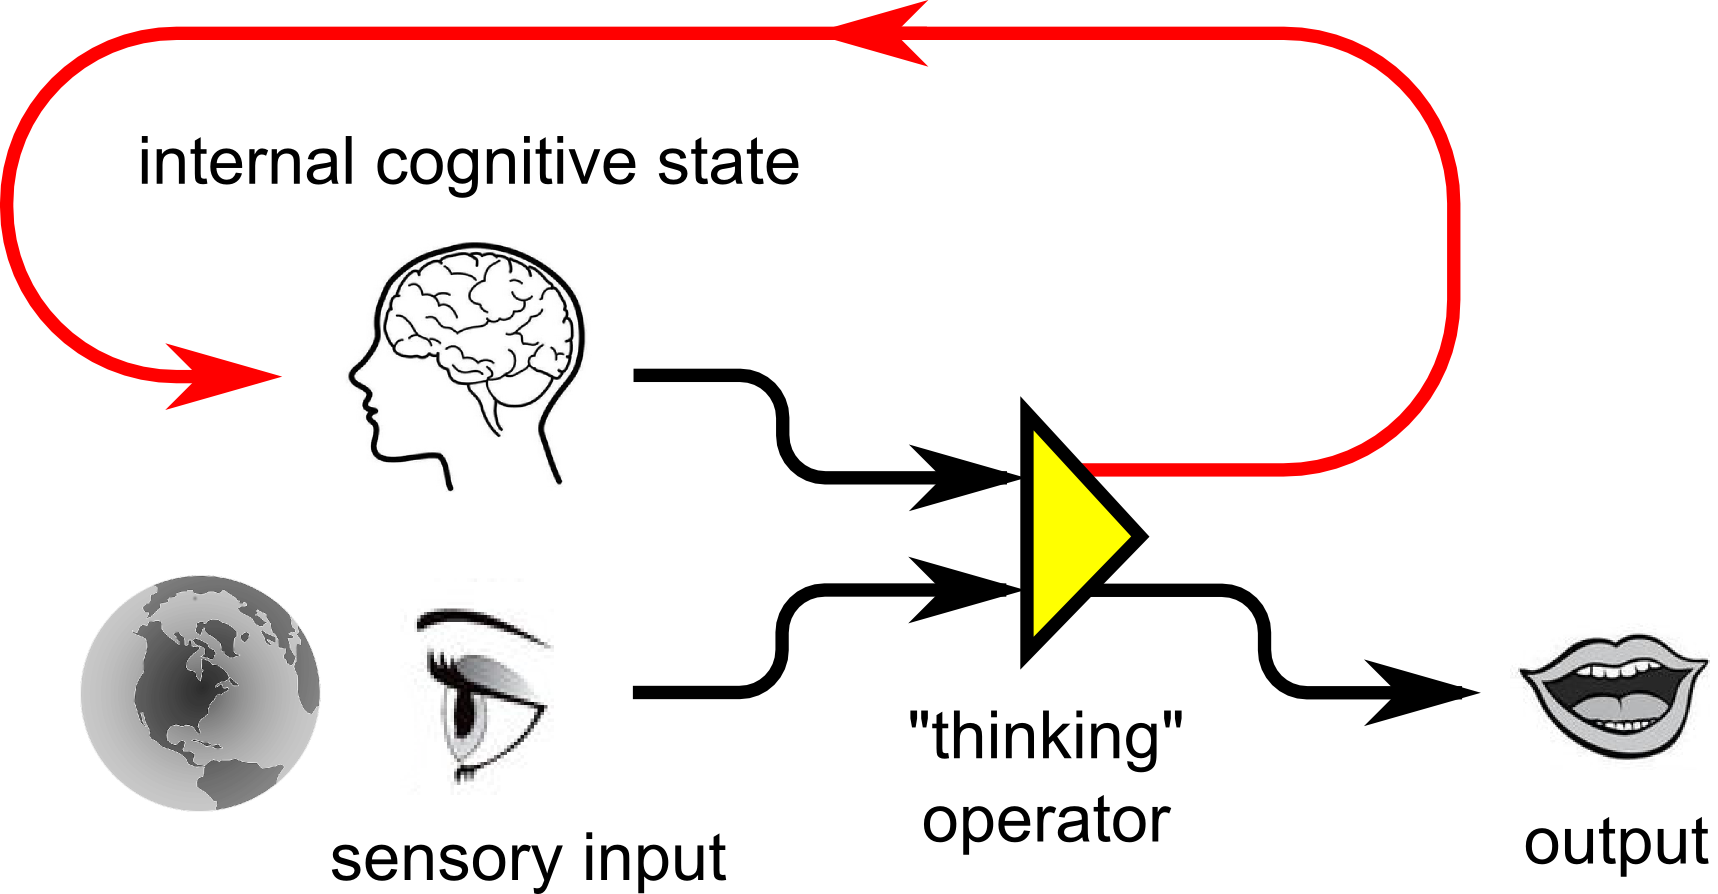
\includegraphics[scale=0.5]{architecture-cartoon.png}}}
\end{equation}

\begin{equation}
\vcenter{\hbox{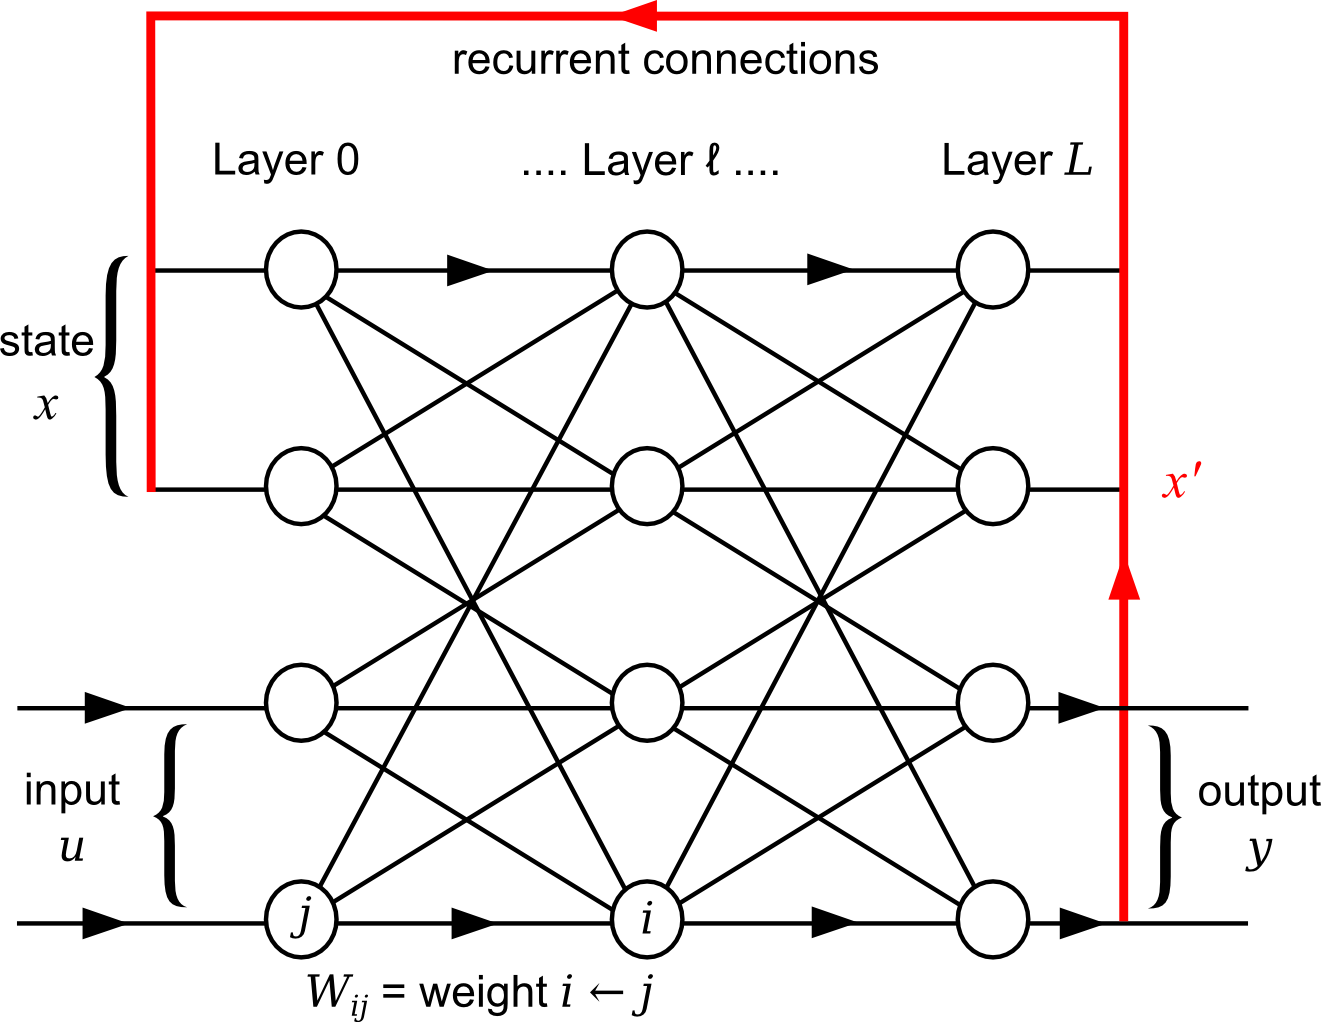
\includegraphics[scale=0.5]{RNN-topology.png}}}
\end{equation}

TO-DO:  The state space $X$ may be too large and we may need an \emp{attention mechanism} to select some parts of $X$ for processing by $R$.  This is the notion of \emp{working memory} in cognitive science.
\begin{equation}
\vcenter{\hbox{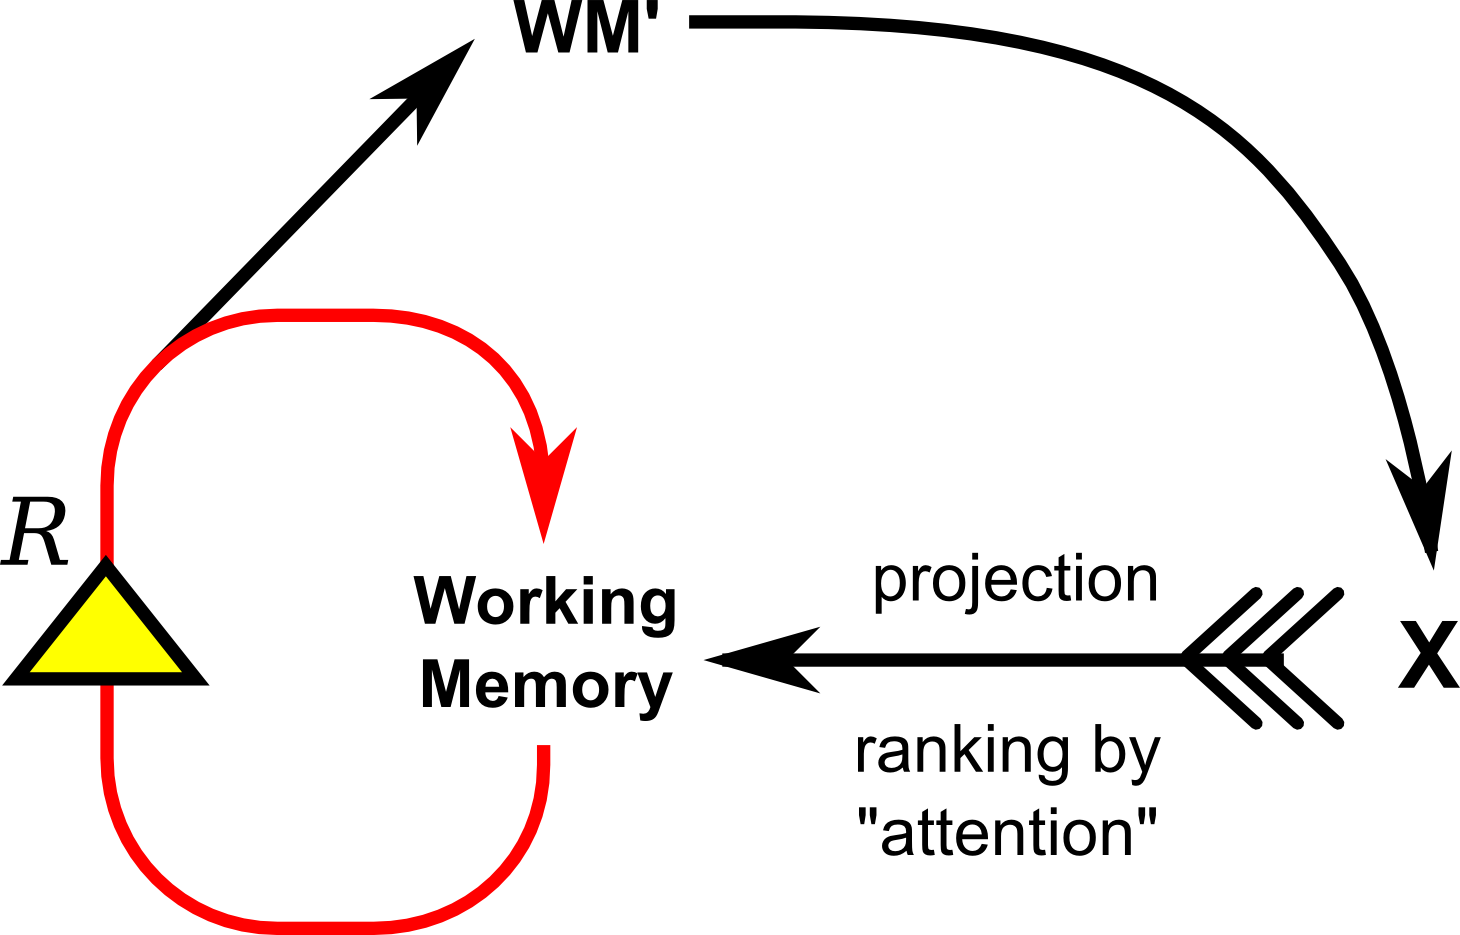
\includegraphics[scale=0.4]{working-memory.png}}}
\end{equation}

\section{Deep Recurrent Learning}

The learning algorithm for $R$ is central to our system.  $R$ learns to recognize input-output pairs $( \vec{x}_0, \vec{x}^* )$.  What makes it special is that $R$ is allowed to iterate a \textit{flexible} number of times before outputting an answer.  In feed-forward learning we simply learn single-pass recognition, whereas in common recurrent learning we train against a \textit{fixed} time sequence.  Here, the time delay between input and output is allowed to stretch arbitrarily.

Suppose the recurrent network $R$ iterates $n$ times:
\begin{equation}
\vec{x}_{t+1} = \overbrace{R \circ R \circ ...}^{n} (\vec{x})
\end{equation}

As $n \rightarrow \infty$, we get the continuous-time version (a differential equation):
\begin{equation}
\frac{d\vec{x}(t)}{dt} = \mathfrak{R}(\vec{x}(t))
\end{equation}

We could run the network $R$ for a long enough time $T$ such that it is highly likely to reach an equilibrium point.  Then:
\begin{equation}
\vec{x}_{T} = \int_0^T \mathfrak{R}(\vec{x}(t)) dt
\end{equation}
and the error:
\begin{equation}
\mathscr{E} = \vec{x}^* - \vec{x}_{T}
\end{equation}
where $\vec{x}^*$ is the target value which is independent of time.
\begin{eqnarray}
\frac{\partial\mathscr{E}}{\partial\vec{W}} &=& - \frac{\partial}{\partial\vec{W}} \int_0^T \mathfrak{R}(\vec{x}(t)) dt \nonumber \\
&=& - \frac{\partial}{\partial\vec{W}} \int_0^T \sigmoid(W_1 \sigmoid(W_2 ... \sigmoid(W_L \vec{x}(t))) dt
\end{eqnarray}

When there are many layers or if the recurrence is too long, back-prop learning becomes ineffective due to the \emp{vanishing gradient} problem.  One solution is to use the \emp{rectifier} activation function:
\begin{equation}
\rectifier (x) = 
\begin{cases}
x, & \mbox{if } x \geq 0 \\
0, & \mbox{otherwise}
\end{cases}
\end{equation}
Since its derivative is piecewise constant, it does not suffer from the vanishing gradient problem.

\subsection{Forward-backward Algorithm}

This is inspired by forward- and backward-chaining in LBAI.  We propagate the state vector from both the initial state $\vec{x}_0$ as well as the final state $\vec{x}^*$.  This bi-directional propagation is added with noise and repeated many times, thus implementing a \emp{stochastic local search}:

\begin{equation}
\vcenter{\hbox{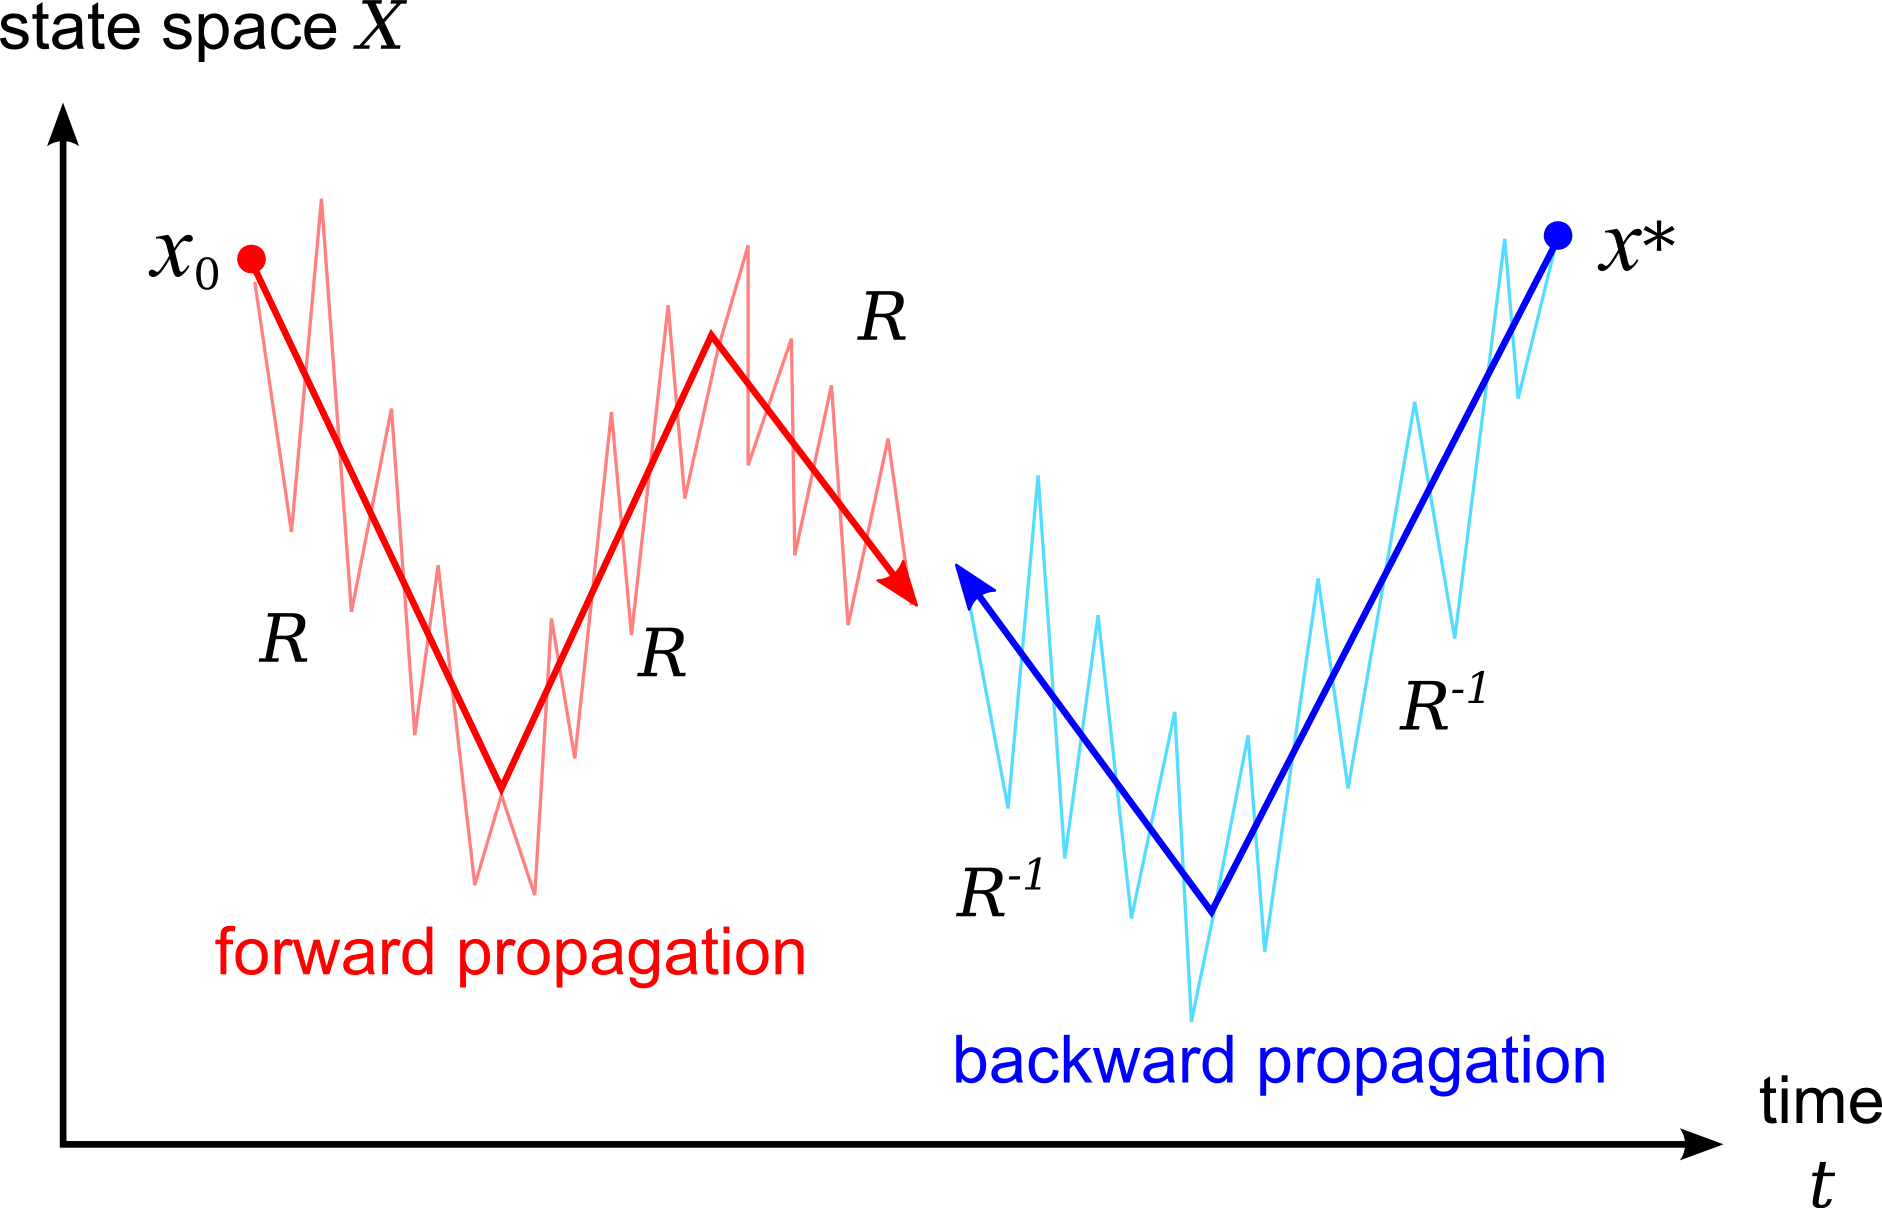
\includegraphics[scale=0.6]{forward-backward-algorithm.png}}}
\end{equation}

When the forward and backward states get close enough, a successful path is found, and we record the gap and the noises along the path, and use them to train $R$ so that this new path would be recognized.

% One key question is how to deal with "don't care" bits?  One answer is that their errors are zero.  But then this is the same as the error for "correct" weights, which seems not well.  There's got to be a way to alter weights when the answer is correct...

% For \# Iteration = 0, output is immediately known, so potentially the training can be done.  But how to convey that all these alterations of weights are \emp{optional}?

% \section{Reinforcement learning}

% ================================== comment out ==================================
\fi

\bibliographystyle{plain} % or number or aaai ...
\bibliography{AGI-book}

\end{document}
